%2multibyte Version: 5.50.0.2960 CodePage: 1252
%\usepackage{mathpazo}


\documentclass[smaller]{beamer}\usepackage[]{graphicx}\usepackage[]{color}
% maxwidth is the original width if it is less than linewidth
% otherwise use linewidth (to make sure the graphics do not exceed the margin)
\makeatletter
\def\maxwidth{ %
  \ifdim\Gin@nat@width>\linewidth
    \linewidth
  \else
    \Gin@nat@width
  \fi
}
\makeatother

\definecolor{fgcolor}{rgb}{0.345, 0.345, 0.345}
\newcommand{\hlnum}[1]{\textcolor[rgb]{0.686,0.059,0.569}{#1}}%
\newcommand{\hlstr}[1]{\textcolor[rgb]{0.192,0.494,0.8}{#1}}%
\newcommand{\hlcom}[1]{\textcolor[rgb]{0.678,0.584,0.686}{\textit{#1}}}%
\newcommand{\hlopt}[1]{\textcolor[rgb]{0,0,0}{#1}}%
\newcommand{\hlstd}[1]{\textcolor[rgb]{0.345,0.345,0.345}{#1}}%
\newcommand{\hlkwa}[1]{\textcolor[rgb]{0.161,0.373,0.58}{\textbf{#1}}}%
\newcommand{\hlkwb}[1]{\textcolor[rgb]{0.69,0.353,0.396}{#1}}%
\newcommand{\hlkwc}[1]{\textcolor[rgb]{0.333,0.667,0.333}{#1}}%
\newcommand{\hlkwd}[1]{\textcolor[rgb]{0.737,0.353,0.396}{\textbf{#1}}}%
\let\hlipl\hlkwb

\usepackage{framed}
\makeatletter
\newenvironment{kframe}{%
 \def\at@end@of@kframe{}%
 \ifinner\ifhmode%
  \def\at@end@of@kframe{\end{minipage}}%
  \begin{minipage}{\columnwidth}%
 \fi\fi%
 \def\FrameCommand##1{\hskip\@totalleftmargin \hskip-\fboxsep
 \colorbox{shadecolor}{##1}\hskip-\fboxsep
     % There is no \\@totalrightmargin, so:
     \hskip-\linewidth \hskip-\@totalleftmargin \hskip\columnwidth}%
 \MakeFramed {\advance\hsize-\width
   \@totalleftmargin\z@ \linewidth\hsize
   \@setminipage}}%
 {\par\unskip\endMakeFramed%
 \at@end@of@kframe}
\makeatother

\definecolor{shadecolor}{rgb}{.97, .97, .97}
\definecolor{messagecolor}{rgb}{0, 0, 0}
\definecolor{warningcolor}{rgb}{1, 0, 1}
\definecolor{errorcolor}{rgb}{1, 0, 0}
\newenvironment{knitrout}{}{} % an empty environment to be redefined in TeX

\usepackage{alltt}
%%%%%%%%%%%%%%%%%%%%%%%%%%%%%%%%%%%%%%%%%%%%%%%%%%%%%%%%%%%%%%%%%%%%%%%%%%%%%%%%%%%%%%%%%%%%%%%%%%%%%%%%%%%%%%%%%%%%%%%%%%%%%%%%%%%%%%%%%%%%%%%%%%%%%%%%%%%%%%%%%%%%%%%%%%%%%%%%%%%%%%%%%%%%%%%%%%%%%%%%%%%%%%%%%%%%%%%%%%%%%%%%%%%%%%%%%%%%%%%%%%%%%%%%%%%%
\usepackage{amssymb}
\usepackage{amsmath}
\usepackage{graphicx}
\usepackage{hyperref}
\usepackage{multimedia}
\usepackage{epstopdf}
\usepackage{color}
\usepackage{tikz}


\setcounter{MaxMatrixCols}{10}
\newtheorem{remark}{Remark}[section]
\newtheorem{proposition}{Proposition}[section]
\newtheorem{interpretation}{Interpretation}[section]
\newtheorem{goal}{Goal}[section]
\newtheorem{statement}{Statement}[section]
\newtheorem{aes}{Aim \& Scope}[section]
\newtheorem{exercise}{Exercise}[section]
\renewcommand{\Pr}{P}

\newcommand{\mbf}[1]{\mathbf{#1}}
\newcommand{\beq}{\begin{equation}}
\newcommand{\eeq}{\end{equation}}
\newcommand{\bea}{\begin{eqnarray}}
\newcommand{\eea}{\end{eqnarray}}
\newcommand{\ba}{\begin{array}}
\newcommand{\ea}{\end{array}}
\newcommand{\bi}{\begin{itemize}}
\newcommand{\ei}{\end{itemize}}
\newcommand{\ben}{\begin{enumerate}}
\newcommand{\een}{\end{enumerate}}
\newcommand{\nn}{\nonumber}
\newcommand{\N}{\mathcal{N}}

\newenvironment{stepenumerate}{\begin{enumerate}[<+->]}{\end{enumerate}}
\newenvironment{stepitemize}{\begin{itemize}[<+->]}{\end{itemize} }
\newenvironment{stepenumeratewithalert}{\begin{enumerate}[<+-| alert@+>]}{\end{enumerate}}
\newenvironment{stepitemizewithalert}{\begin{itemize}[<+-| alert@+>]}{\end{itemize} }
\usetheme{Madrid}


%%%%%%%%%%%%%%%%%%%%%%%%%%%%%%%%%%%%%%%%%%%%%%%%%%%%%%%%%%%%%%%%%%%%%%%%%%%%%%%
% GSEM COLORS
%%%%%%%%%%%%%%%%%%%%%%%%%%%%%%%%%%%%%%%%%%%%%%%%%%%%%%%%%%%%%%%%%%%%%%%%%%%%%%%
\definecolor{darkGSEM}{RGB}{70,95,127}
\definecolor{darkGSEM2}{RGB}{40,80,150}
\definecolor{GSEM}{RGB}{96,121,153} % GSEM 10% lighter

%%% Global colors
\setbeamercolor*{palette primary}{use=structure,fg=white,bg=darkGSEM}
\setbeamercolor*{palette quaternary}{use=structure,fg=white,bg=darkGSEM!90}
\setbeamercolor{frametitle}{fg=white,bg=GSEM!80}

%%% TOC colors
\setbeamercolor{section in toc}{fg=darkGSEM}

%%% itemize colors
\setbeamertemplate{itemize items}[circle]
\setbeamercolor{itemize item}{fg=darkGSEM2}
\setbeamercolor{itemize subitem}{fg=darkGSEM2}
\setbeamercolor{itemize subsubitem}{fg=darkGSEM2}


%%% enumerate colors
\setbeamercolor{item projected}{fg=white,bg=GSEM}
\setbeamertemplate{enumerate item}{\insertenumlabel.}
\setbeamercolor{enumerate item}{fg=darkGSEM2}
\setbeamercolor{enumerate subitem}{fg=darkGSEM2}
\setbeamercolor{enumerate subsubitem}{fg=darkGSEM2}


\AtBeginSection[]
{
  \begin{frame}
    \frametitle{Outline}
    \tableofcontents[currentsection]
  \end{frame}
}

\AtBeginSubsection[]
{
  \begin{frame}
    \frametitle{Outline}
    \tableofcontents[currentsubsection]
  \end{frame}
}



%%%%%%%%%%%%%%%%%%%%%%%%%%%%%%%%%%%%%%%%%%%%%%%%%%%%%%%%%%%%%%%%%%%%%%%%%%%%%%%%
% R Chunk Options and Packages
%%%%%%%%%%%%%%%%%%%%%%%%%%%%%%%%%%%%%%%%%%%%%%%%%%%%%%%%%%%%%%%%%%%%%%%%%%%%%%%%




%%%%%%%%%%%%%%%%%%%%%%%%%%%%%%%%%%%%%%%%%%%%%%%%%%%%%%%%%%%%%%%%%%%%%%%%%%%%%%%%
\IfFileExists{upquote.sty}{\usepackage{upquote}}{}
\begin{document}

\title[S110015]{Probability 1}
\subtitle{Chapter 05 : Continuous Random Variables - Part 1}
\author[Flores-Agreda, La Vecchia]{Dr. Daniel Flores-Agreda, \\[0.5em] \tiny{(based on the notes of Prof. Davide La Vecchia)}}
\date{Spring Semester 2021}

\begin{frame}
\titlepage
\end{frame}


\begin{frame}{Objectives}

\end{frame}

\begin{frame}{Outline}
\tableofcontents
\end{frame}


%%%%%%%%%%%%%%%%%%%%%%%%%%%%%%%%%%%%%%%%%%%%%%%%%%%%%%%%%%%%%%%%%%%%%%%%%%%%%%%
\subsection{Gaussian or ``Normal'' Distribution}
%%%%%%%%%%%%%%%%%%%%%%%%%%%%%%%%%%%%%%%%%%%%%%%%%%%%%%%%%%%%%%%%%%%%%%%%%%%%%%%

\begin{frame}{\subsecname}
  
  Last class we said that, the Normal PDF is \textbf{Symmetric}
  
  $$\phi_{(\mu,\sigma)}(-x) = \phi_{(\mu,\sigma)}(x)$$
  
\begin{knitrout}
\definecolor{shadecolor}{rgb}{0.969, 0.969, 0.969}\color{fgcolor}

{\centering 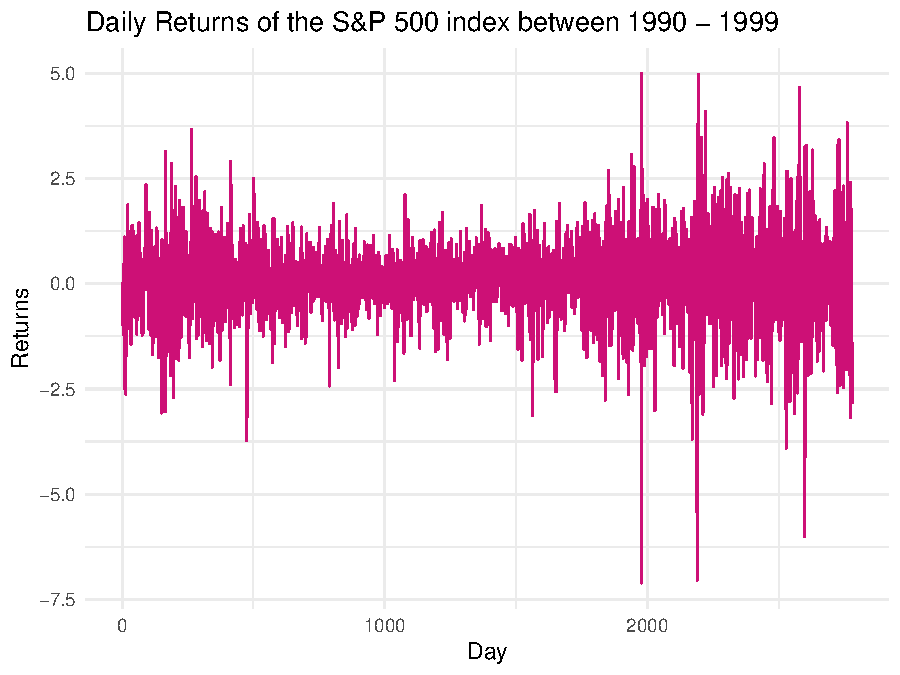
\includegraphics[width=0.5\linewidth]{figure/unnamed-chunk-2-1} 

}



\end{knitrout}
  
\end{frame}


\begin{frame}{\subsecname}
  
  Of course, the \textbf{Standard} Normal PDF is also \textbf{Symmetric}
  
  $$\phi(-x) = \phi(x)$$
\begin{knitrout}
\definecolor{shadecolor}{rgb}{0.969, 0.969, 0.969}\color{fgcolor}

{\centering 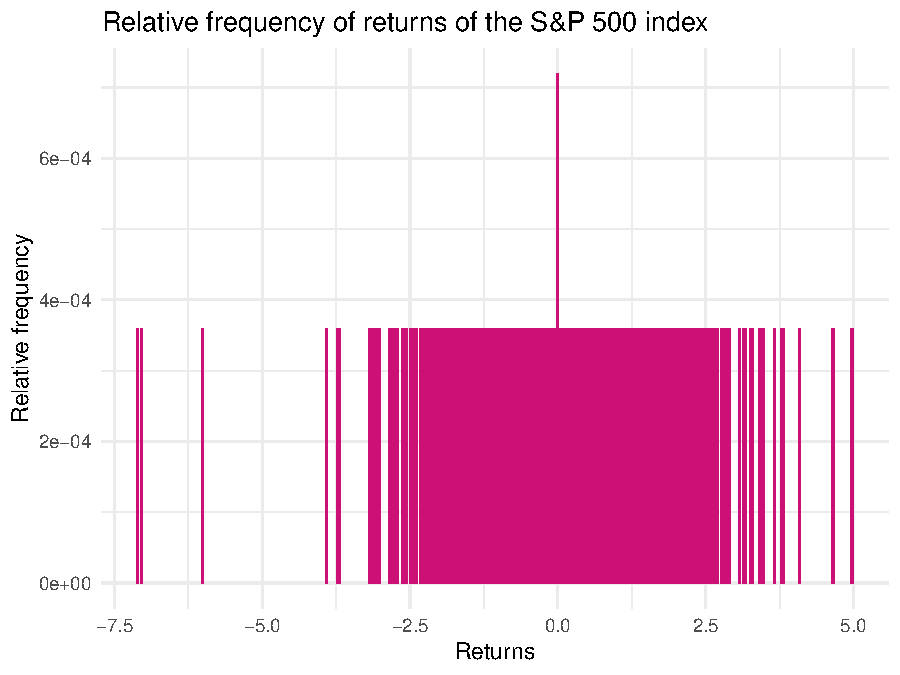
\includegraphics[width=0.5\linewidth]{figure/unnamed-chunk-3-1} 

}



\end{knitrout}
\end{frame}

\begin{frame}{\subsecname}
  
  \textbf{Symmetry} of the PDF implies that the CDF can be computed as 
  
  $$\Phi(-x) = 1-\Phi(x)$$


\only<1-1>{
\begin{knitrout}
\definecolor{shadecolor}{rgb}{0.969, 0.969, 0.969}\color{fgcolor}

{\centering 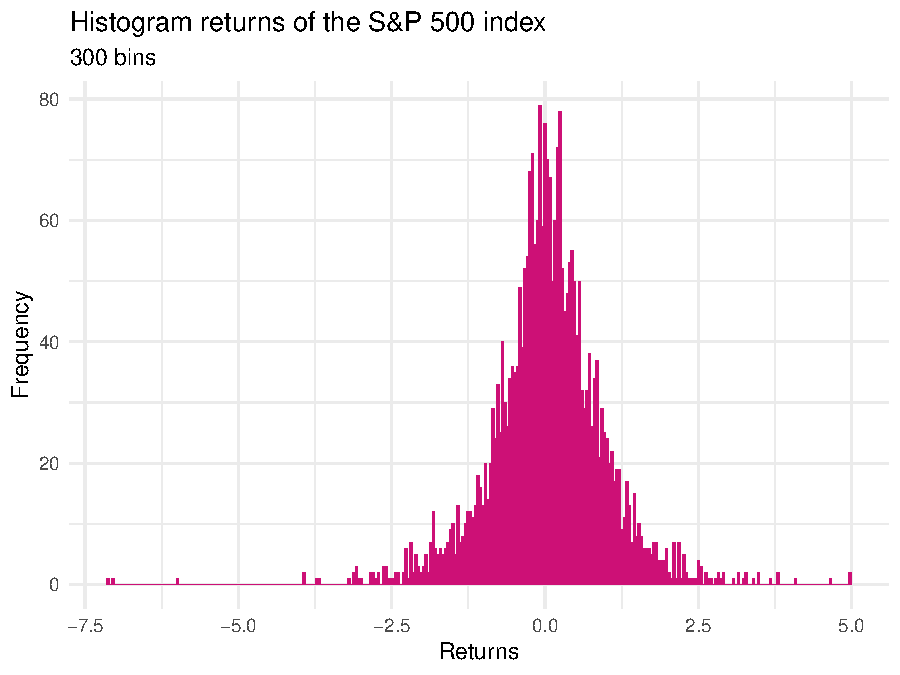
\includegraphics[width=0.5\linewidth]{figure/unnamed-chunk-5-1} 

}



\end{knitrout}
}
\only<2-2>{
\begin{knitrout}
\definecolor{shadecolor}{rgb}{0.969, 0.969, 0.969}\color{fgcolor}

{\centering 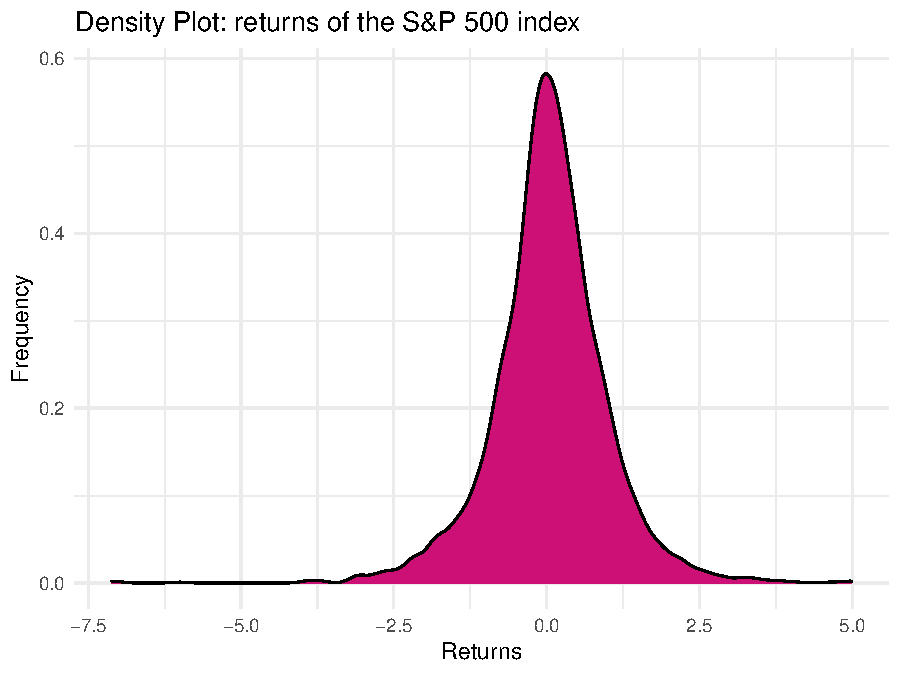
\includegraphics[width=0.5\linewidth]{figure/unnamed-chunk-6-1} 

}



\end{knitrout}
}
\only<3-3>{
\begin{knitrout}
\definecolor{shadecolor}{rgb}{0.969, 0.969, 0.969}\color{fgcolor}

{\centering 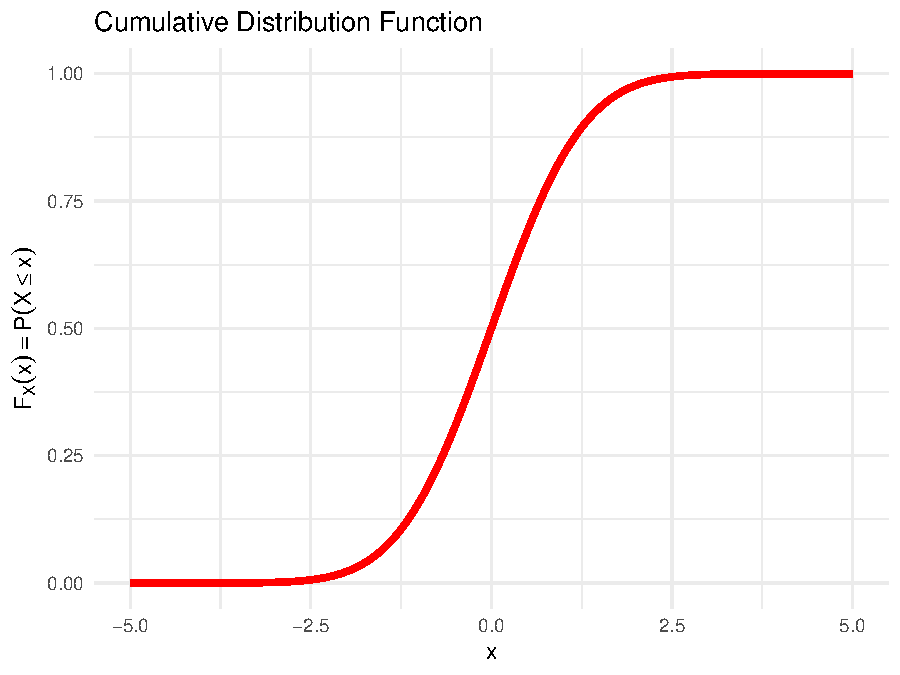
\includegraphics[width=0.5\linewidth]{figure/unnamed-chunk-7-1} 

}



\end{knitrout}
}
\end{frame}


\begin{frame}{\subsecname}
  % Thus statements about a Normal random variable can always be translated into equivalent statements about a standard Normal random variable, and vice versa.
  
  We can \textbf{shift and scale} any Normal Random Variable $X$ and reach a \textbf{Standard Normal Random Variable} $Z$ 
  
  $$X\sim \N\left( \mu ,\sigma ^{2}\right)\Longleftrightarrow Z=\frac{\left( X-\mu \right) }{\sigma }\sim \N\left( 0,1\right)$$
  
  \begin{itemize}
  \item We can always transform from $X$ to $Z$ 
  \begin{equation*}
  Z=\frac{X-\mu }{\sigma } \ (\text{for the random variable}) \quad\mbox{and}\quad z=\frac{x-\mu }{\sigma }\,  \ (\text{for its values}) ,
  \end{equation*}
  \item and return back to $X$ by a `re-scaling' and `re-shifting':%
  \begin{equation*}
  X=\sigma Z+\mu  \ (\text{for the random variable}) \quad\mbox{and}\quad x=\sigma z+\mu\, \ (\text{for its values}) .
  \end{equation*}
  \end{itemize}
Statements about a Normal Random Variable can always be translated into equivalent statements about a standard Normal Random Variable, (and vice-versa).
\end{frame}

\begin{frame}{\subsecname}
  In particular, the \textbf{CDF of any Normal Random Variable} $X\sim \N(\mu, \sigma^2)$, can 
  be \textbf{computed} with a \textbf{Standard CDF}
  
  \begin{align*}
  P(\{ X\leq x\}) &= 
  P\left(\left\{\underbrace{\frac{X-\mu}{\sigma}}_Z\leq \underbrace{\frac{x-\mu}{\sigma}}_{z}\right\}\right) \\
  &= P(\{ Z\leq z\}) \\
  P(\{ X\leq x\})&= \Phi(z)
  \end{align*}
\end{frame}

\begin{frame}{\subsecname}
Moreover, we can also compute the probabilities of any interval for $X\sim \N\left( \mu ,\sigma ^{2}\right)$ with the \textbf{Standard CDF}

\begin{align*}
  \Pr(\{x_1<X\leq x_2\}) &= 
  \Pr\left(\left\{\frac{x_1-\mu}{\sigma}<\frac{X-\mu}{\sigma}\leq \frac{x_2-\mu}{\sigma}\right\}\right) \\ 
  &= \Pr(\{z_1<Z\leq z_2\})\\
  &= \Pr(\{Z\leq z_2\}) - \Pr(\{Z\leq z_1\})\\
  \Pr(\{x_1<X\leq x_2\}) &= \Phi(z_2)-\Phi(z_1)
\end{align*}
where $z_1=(x_1-\mu)/\sigma$ and $z_2=(x_2-\mu)/\sigma$.
\end{frame}

\begin{frame}{\subsecname}
$$\Pr(\{z_1<Z\leq z_2\}) = \Pr(\{Z\leq z_2\}) - \Pr(\{Z\leq z_1\})=\Phi(z_2)-\Phi(z_1)$$

\only<2-2>{
\begin{knitrout}
\definecolor{shadecolor}{rgb}{0.969, 0.969, 0.969}\color{fgcolor}

{\centering 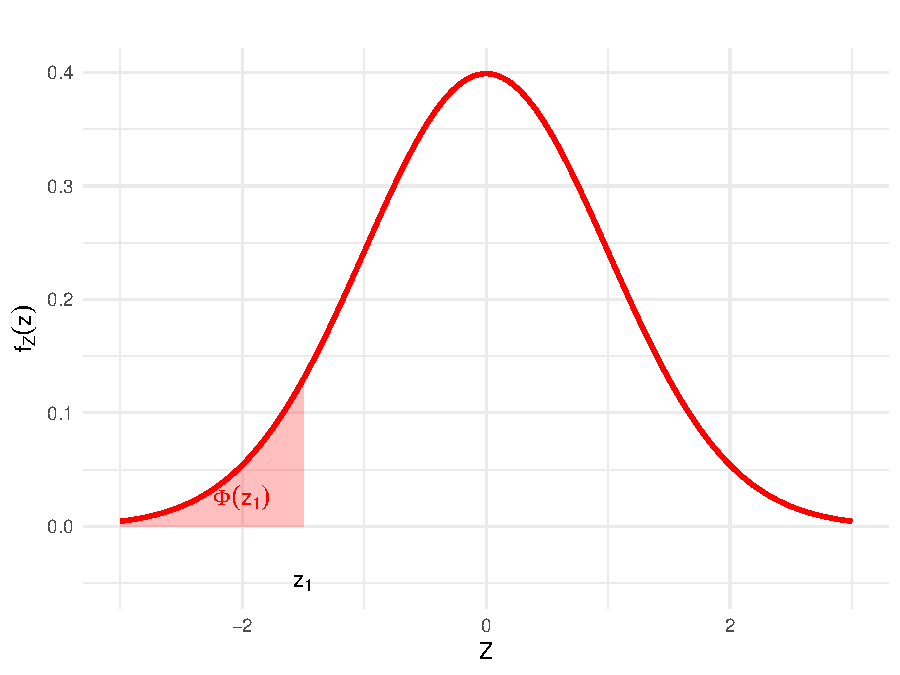
\includegraphics[width=0.5\linewidth]{figure/unnamed-chunk-9-1} 

}



\end{knitrout}
}
\only<3-3>{
\begin{knitrout}
\definecolor{shadecolor}{rgb}{0.969, 0.969, 0.969}\color{fgcolor}

{\centering 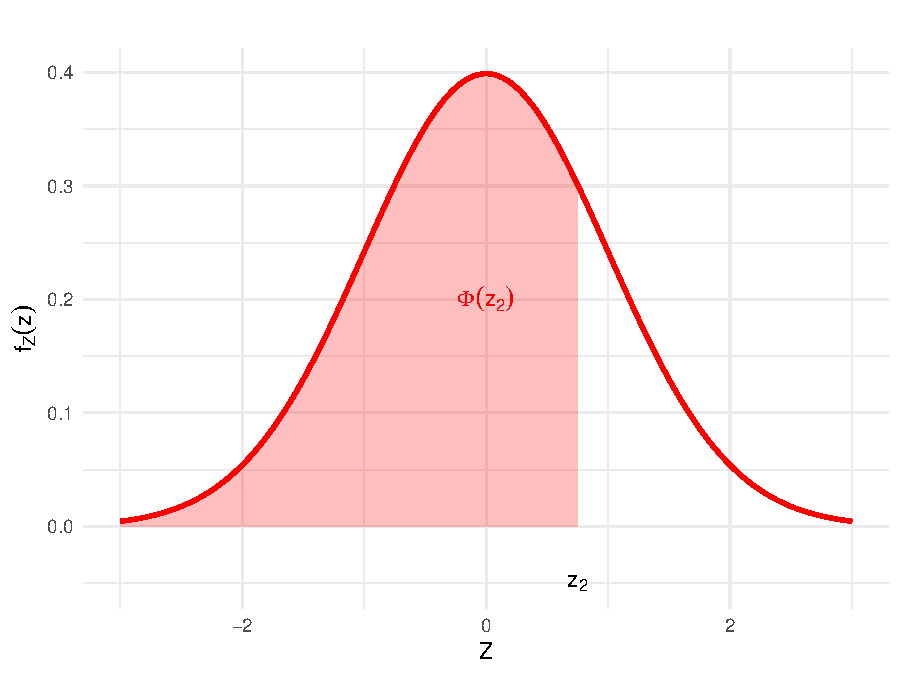
\includegraphics[width=0.5\linewidth]{figure/unnamed-chunk-10-1} 

}



\end{knitrout}
}
\only<4-4>{
\begin{knitrout}
\definecolor{shadecolor}{rgb}{0.969, 0.969, 0.969}\color{fgcolor}

{\centering 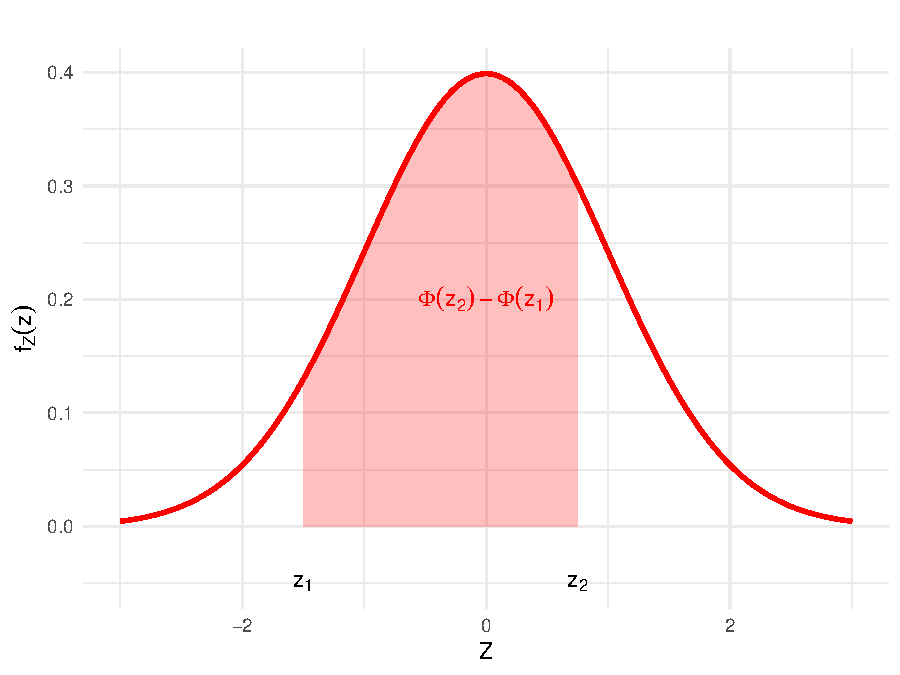
\includegraphics[width=0.5\linewidth]{figure/unnamed-chunk-11-1} 

}



\end{knitrout}
}
\end{frame}


\begin{frame}{\subsecname}
The integral that defines the CDF of the standard normal:
  $$
  \Pr(\{Z\leq z\})=\Phi(z)=\int_{-\infty}^z\phi(s)ds
  $$
  \textbf{does not have} a closed-form expression.

  \begin{itemize}
    \item It can be \textbf{approximated} using a computer.
    \item We can rely on \textbf{Standard Normal Tables}, which show the values of $\Phi(z)$ for $z\geq 0$
  \end{itemize}
  
  \begin{remark}
     We can obtain $\Phi(z)$ for $z < 0$ by symmetry of $\phi(z)$ which, again, entails:
     $$\Phi(-z)=1-\Phi(z)$$
  \end{remark}
\end{frame}

\begin{frame}{\subsecname}
Description of the values contained in the table:
  \begin{figure}[ptb]\centering
  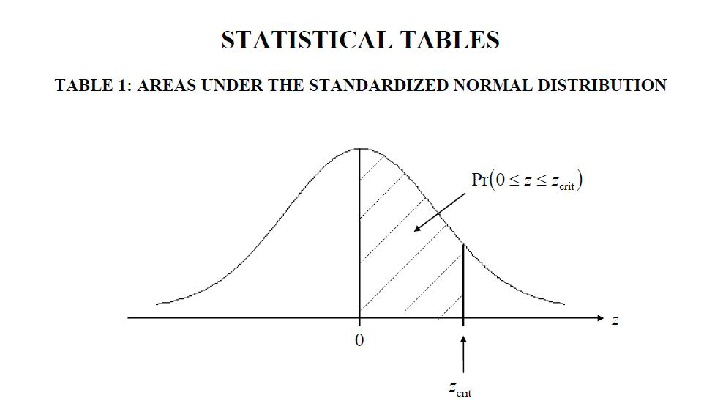
\includegraphics[width=0.95\textwidth,height=0.75\textheight]{img/bell_curve__5.pdf}
  \end{figure}
\end{frame}


\begin{frame}{\subsecname}
Contents of the table
  \begin{figure}[ptb]\centering
  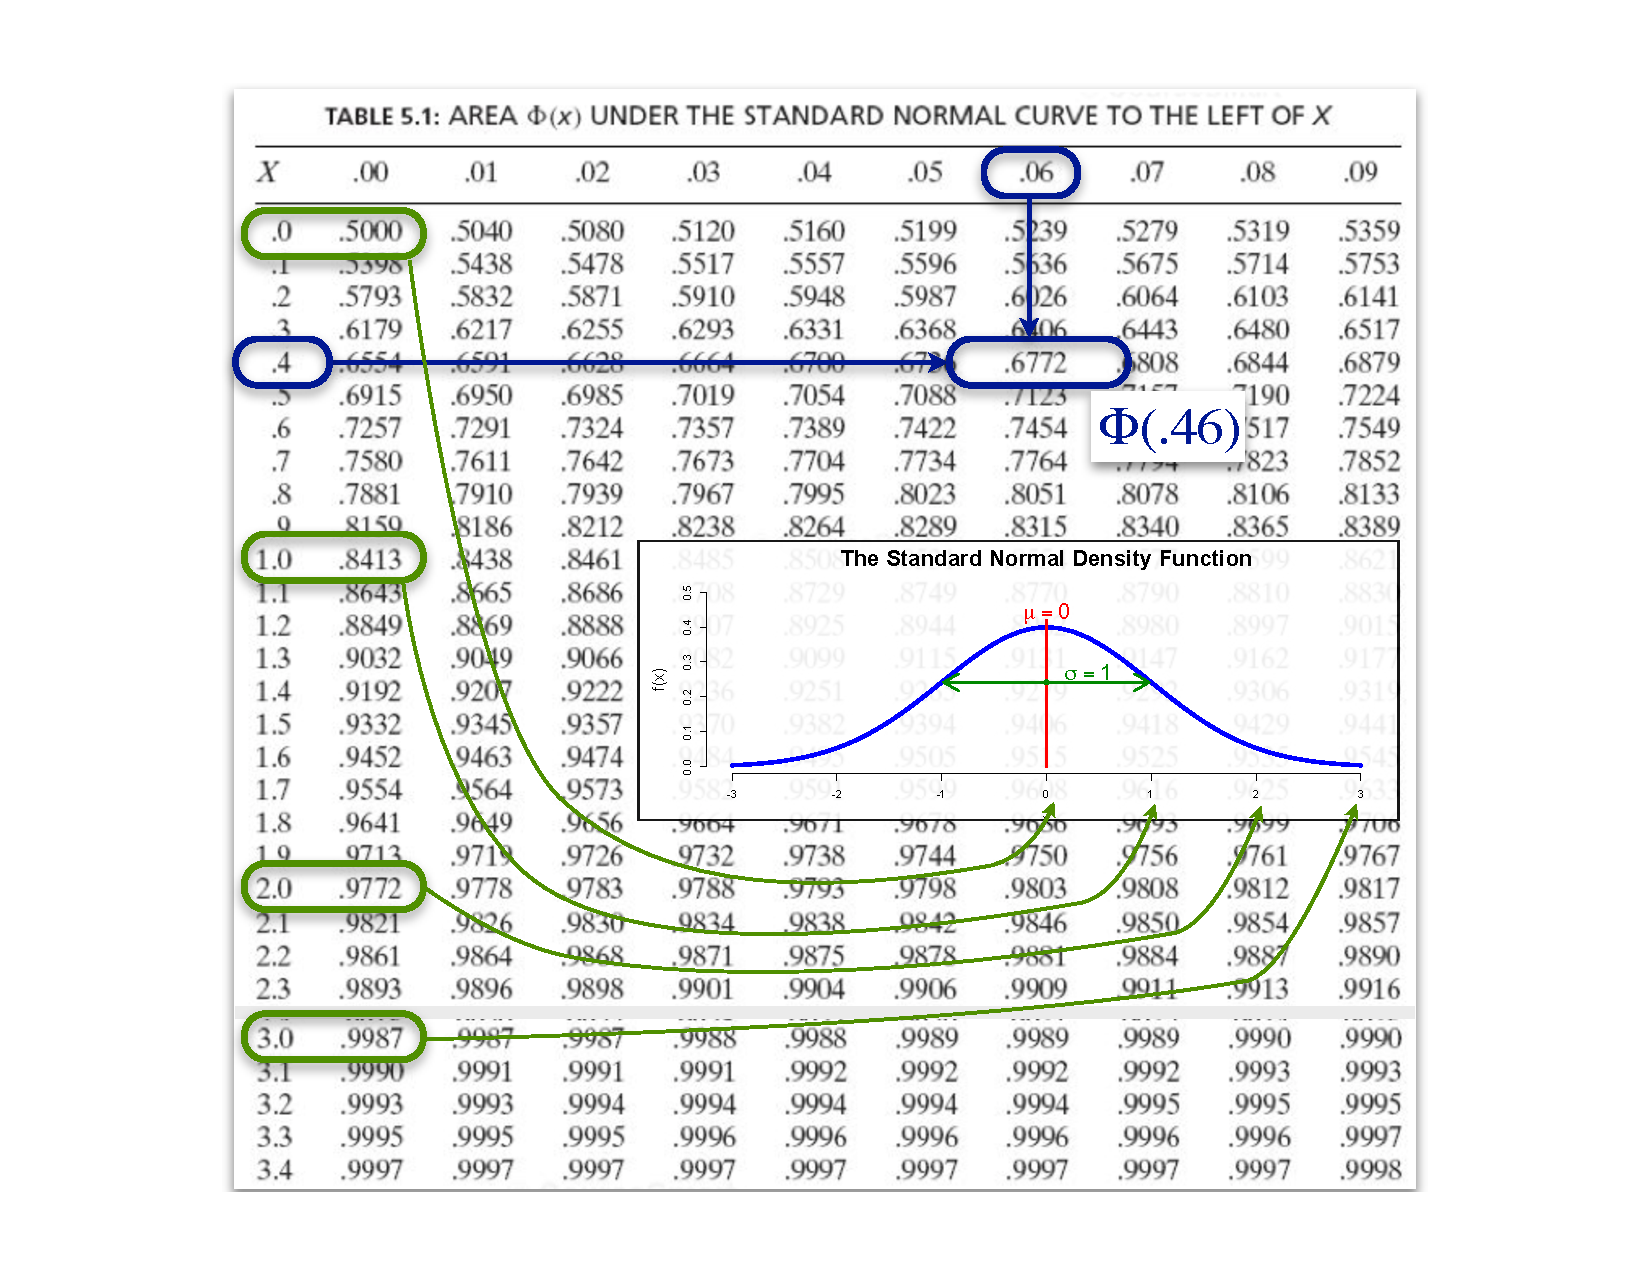
\includegraphics[width=0.9\textwidth,height=0.95\textheight]{img/myTableGauss.pdf}
  \end{figure}
\end{frame}
  
\begin{frame}{\subsecname}
  One can use these tables to compute integrals/probabilities of the type:
  \begin{figure}[ptb]\centering
  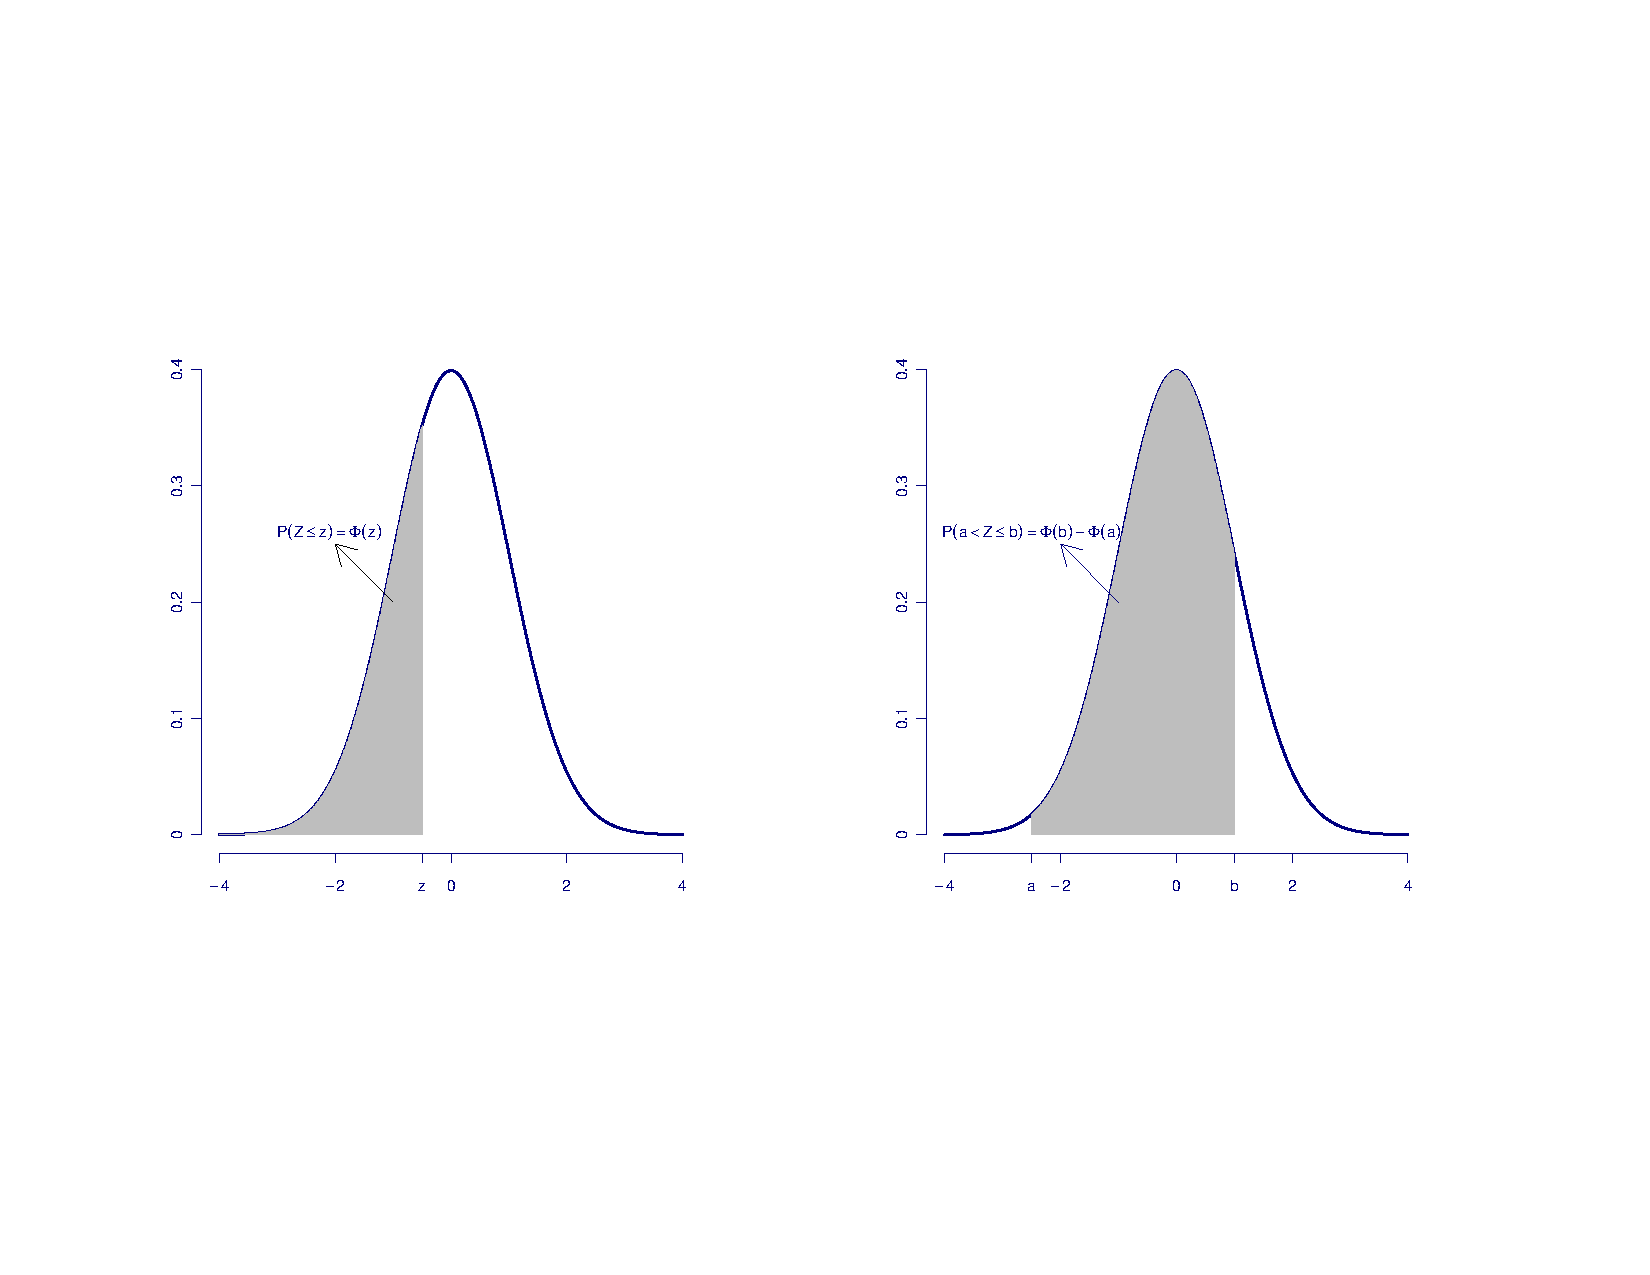
\includegraphics[height=2in, width=4in]{img/CDF_pr.pdf}%
  \end{figure}
\end{frame}

\begin{frame}{\subsecname}
%\frametitle{Standard Normal Tables}

\begin{example}[Prob of $Z$]
\begin{footnotesize}
  \begin{tabular}{ll}
  $P(\{Z\leq 1\})$ & $\approx0.8413\bigskip $ \\
  $P(\{Z\leq 1.96\})$ & $\approx0.9750\bigskip $ \\
  $P(\{Z\geq 1.96\})$ & $=1-P(\{Z\leq 1.96\})$ $\approx1-0.9750=0.0250\bigskip $\\
  $P(\{Z\geq -1\})$ & $=P(\{Z\leq 1\})\approx0.8413\bigskip $ \\
  $P(\{Z\leq -1.5\})$ & $=P(\{Z\geq 1.5\}) =1-P(\{Z\leq 1.5\})$ $\approx1-0.9332=0.0668$%
  \end{tabular}
  \end{footnotesize}
  \end{example}
\end{frame}%

\begin{frame}{\subsecname}
  %\frametitle{Standard Normal Tables}
  
  \begin{example}[continued]
  \begin{footnotesize}
  \begin{tabular}{ll}
  & $P(\{0.64\leq Z\leq 1.96\})=$ \\
  & $P(\{Z\leq 1.96\})-P(\{Z\leq 0.64\})$ \\
  & $\approx 0.9750-0.7389=0.2361\bigskip $ \\
  & $P(\{-0.64\leq Z\leq 1.96\})$ \\
  & $=P(\{Z\leq 1.96\})-P(\{Z\leq -0.64\})$ \\
  & $=P(\{Z\leq 1.96\})-(1-P(\{Z\leq 0.64\}))$ \\
  & $\approx0.9750-(1-0.7389)=0.7139\bigskip $ \\
  & $P(\{-1.96\leq Z\leq -0.64\})$ \\
  & $=P(\{0.64\leq Z\leq 1.96\})$ \\
  & $\approx0.2361$%
  \end{tabular}
  \end{footnotesize}
  \end{example}
\end{frame}%

\begin{frame}{\subsecname}
  %\frametitle{Some properties of the Normal distribution}
  \begin{figure}[ptb]\centering
  \ \hspace{0.6cm} One $\sigma$ \hspace{2.4cm} Two $\sigma$s \hspace{2.5cm} Three $\sigma$s \hspace{3cm}
  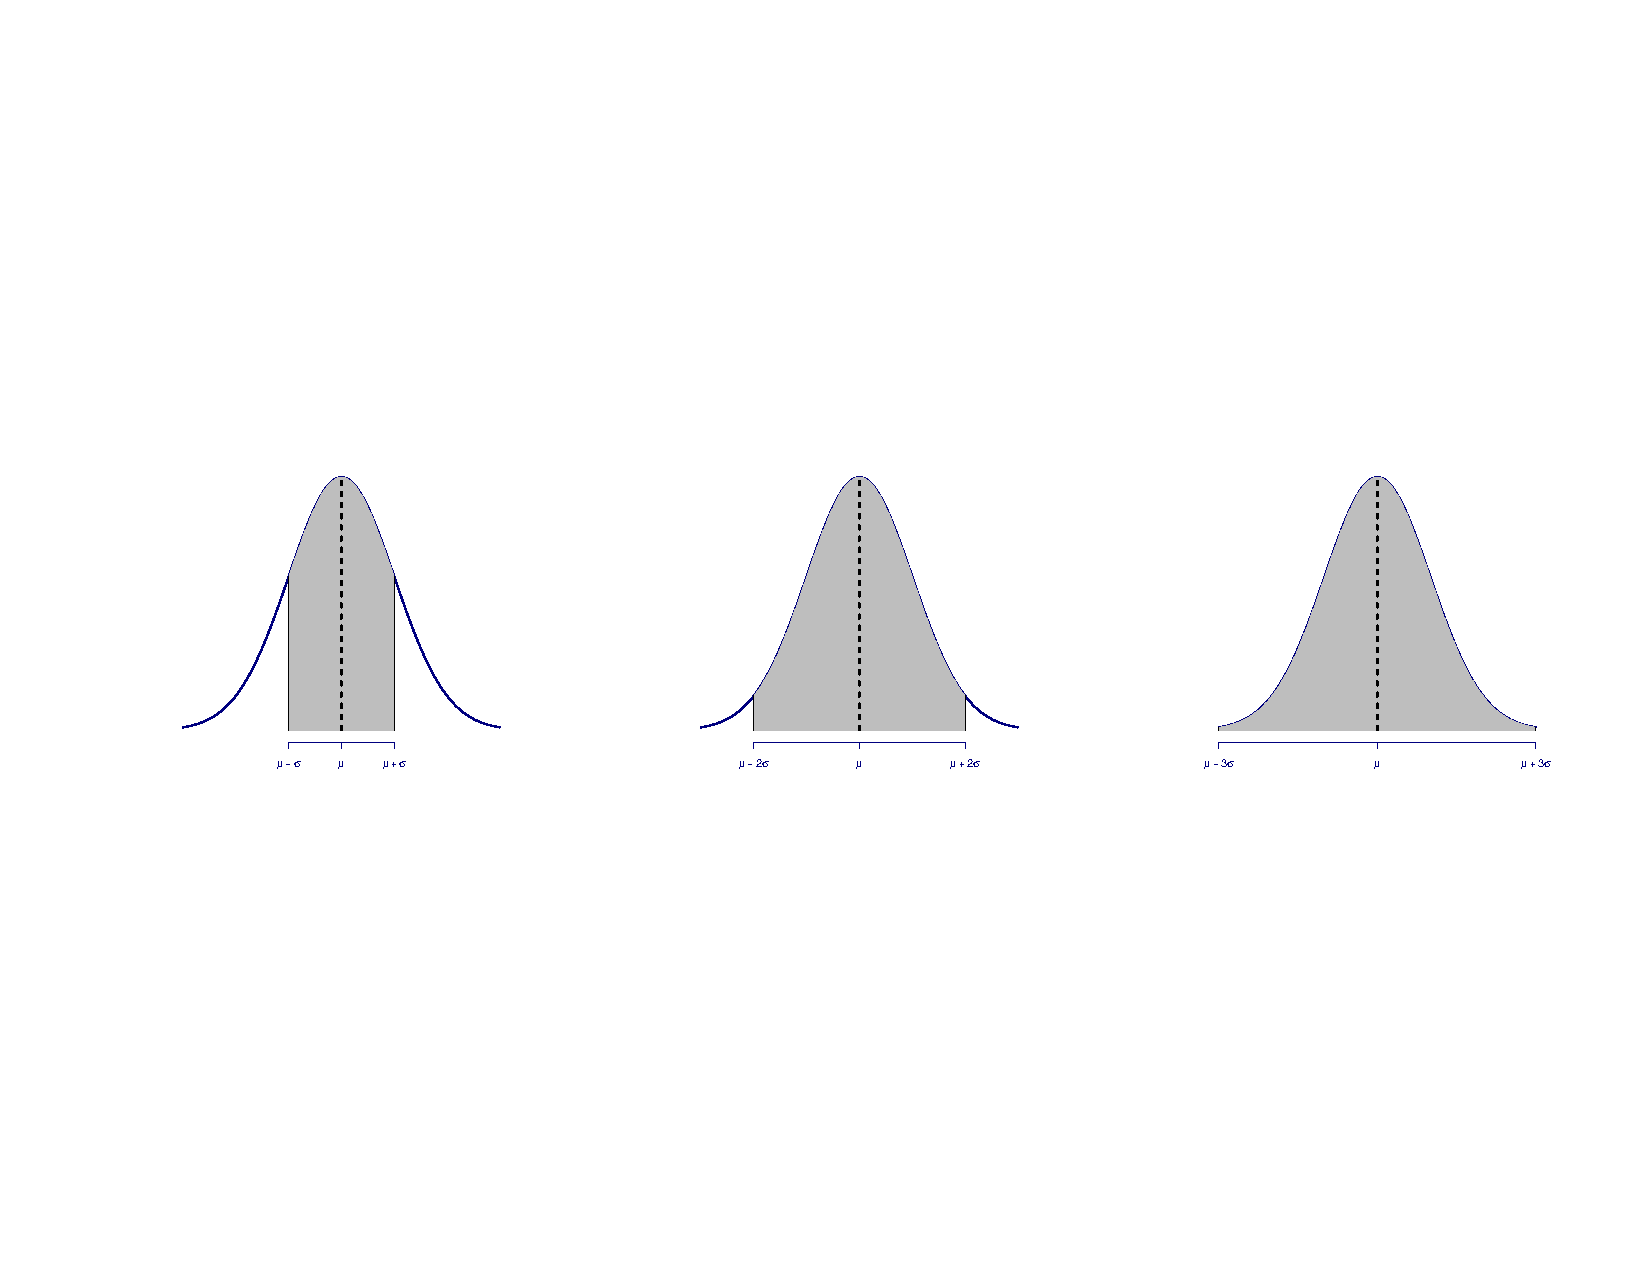
\includegraphics[height=1.5in, width=4.5in]{img/Areas_Normal.pdf}%
  \end{figure}%
  The shaded areas under the pdfs are (approximately) equivalent to $0.683$, $0.954$ and $0.997$,
  respectively. So we state  the following ....
\end{frame}

\begin{frame}{\subsecname}
  %\frametitle{Some properties of the Normal distribution}
  \textbf{... rule `68 -- 95 -- 99.7'}: \\ \bigskip
  
  
  If $X$ is a Normal random variable, $X \sim \N(\mu, \sigma^2)$, its realization has approximately a probability of \\ \bigskip
  
  \begin{tabular}{llll}
  $\bullet$
  &
  $68 \, \%$
  &
  \mbox{of being in the interval}
  &
  $\lbrack \mu - \sigma, \, \mu + \sigma \rbrack$;\\[0.2cm]
  $\bullet$
  &
  $95 \, \%$
  &
  \mbox{of being in the interval}
  &
  $\lbrack \mu - 2 \, \sigma, \, \mu + 2 \, \sigma \rbrack$;\\[0.2cm]
  $\bullet$
  &
  $99.7 \, \%$
  &
  \mbox{of being in the interval}&
  $\lbrack \mu - 3 \, \sigma, \, \mu + 3 \, \sigma \rbrack$.\\[0.2cm]
  \end{tabular}
\end{frame}


\begin{frame}{\subsecname}
  %\frametitle{Some properties of the Normal distribution}
  
  \begin{stepitemize}
  \item For $X\sim \N\left( \mu ,\sigma ^{2}\right) $
  \begin{equation*}
  E\left[ X\right] =\mu \text{ and }Var\left( X\right) =\sigma ^{2}.
  \end{equation*}
  
  \item If $a$ is a number, then
  \begin{eqnarray*}
  X+a &\sim &\N\left( \mu +a,\sigma ^{2}\right) \\
  aX &\sim &\N\left( a\mu ,a^{2}\sigma ^{2}\right).
  \end{eqnarray*}
  
  \item If $X\sim \N\left( \mu ,\sigma ^{2}\right) $ and $Y\sim \N\left( \alpha
  ,\delta ^{2}\right) $, and $X$ and $Y$ are \textbf{independent} then%
  \begin{equation*}
  X+Y\sim \N\left( \mu +\alpha ,\sigma ^{2}+\delta ^{2}\right).
  \end{equation*}
  \end{stepitemize}
\end{frame}


\begin{frame}{\subsecname}
%\frametitle{The sum of two independent Normals}
  \begin{figure}[ptb]\centering
  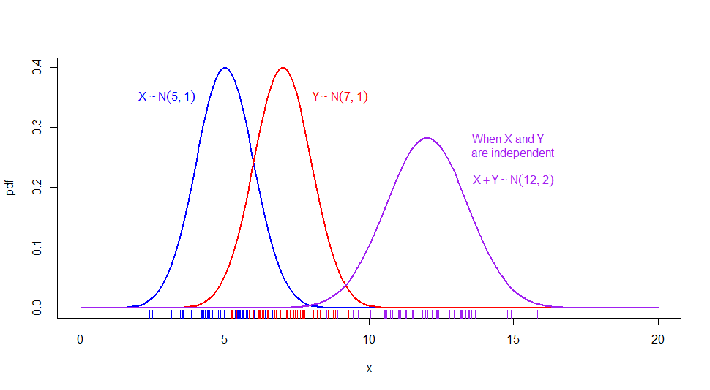
\includegraphics[width=0.95\textwidth,height=0.7\textheight]{img/sum_of_two_independent_normals_with_rug__1.pdf}%
  \end{figure}
  Locations of $n=30$ sampled values of $X,$ $Y$, and $X+Y$ shown as tick marks under each respective density.
\end{frame}


\begin{frame}{\subsecname}


%\frametitle{Normal: an example}

\begin{example}

On the highway A2 (in the Luzern area), the speed is limited to $80$ $km/h$. A radar measures the speeds of all the cars.
Assuming that the registered speeds are distributed according to a Normal law with mean $72$ $km/h$ and standard error $8$ $km/h$: \vspace{0.2cm}
\begin{enumerate}
  \item what is the proportion of the drivers who will have to pay a penalty for high speed? \vspace{0.2cm}
  \item knowing that in addition to the penalty, a speed higher than $30$ $km/h$ (over the max allowed speed) implies a withdrawal of the driving license, what is the proportion of the drivers who  will lose their driving license among those who will have a to pay a fine?
\end{enumerate}

\end{example}
\end{frame}



\begin{frame}{\subsecname}
  \begin{example}[continued]
  Let $X$ be the random variable expressing the registered speed: $X \sim \mathcal{N}(72,64)$.
    \begin{enumerate}
    \item Since a driver has to pay if its speed is above  $80$ $km/h$, the proportion of drivers paying a penalty is expressed  through $P(X>80)$:
    \begin{equation*}
    P(X>80)= P\left(Z>\frac{80-72}{8} \right)=1-\Phi(1) \simeq 16 \%
    \end{equation*}
    where $Z \sim \mathcal{N}(0,1)$.
    \item We are looking for the conditional probability of a recorded speed greater than 110 \underline{given that} the driver has had already to pay a fine:
    \begin{eqnarray*}
    P(X>110 \vert X>80) &=&  \frac{P(\{X>110\} \bigcap \{X>80\})}{P(X>80)} \\
    &=& \frac{P(X>110)}{P(X>80)} = \frac{1- \Phi((110-72)/8)}{1-\Phi(1)}\approx \frac{0}{16\%}\simeq 0.
    \end{eqnarray*}
    \end{enumerate}
  \end{example}
\end{frame}


%%%%%%%%%%%%%%%%%%%%%%%%%%%%%%%%%%%%%%%%%%%%%%%%%%%%%%%%%%%%%%%%%%%%%%%%%%%%%%%%
\subsection{The Chi-squared distribution}
%%%%%%%%%%%%%%%%%%%%%%%%%%%%%%%%%%%%%%%%%%%%%%%%%%%%%%%%%%%%%%%%%%%%%%%%%%%%%%%%

\begin{frame}{\subsecname}
  \begin{definition}
  If $Z_{1},Z_{2},\ldots ,Z_{n}$ are independent standard Normal random
  variables, then%
  \begin{equation*}
  X=Z_{1}^{2}+Z_{2}^{2}+\cdots +Z_{n}^{2}
  \end{equation*}%
  has a chi-squared distribution with $n$ degrees of freedom. Write as $X\sim \chi ^{2}(n)$.
  \end{definition}

  $X\sim \chi ^{2}(n)$ can take only \textbf{positive }values. Moreover, expected value and variance, for $X\sim \chi ^{2}(n)$, are:
  \begin{eqnarray*}
  E\left[ X\right] &=&n \\
  Var\left( X\right) &=&2n
  \end{eqnarray*}

  If $X\sim \chi ^{2}(n)$ and $Y\sim \chi ^{2}(m)$ are \textbf{%
  independent} then $X+Y\sim \chi ^{2}(n+m)$.
\end{frame}

\begin{frame}{\subsecname}

\begin{figure}[ptb]\centering
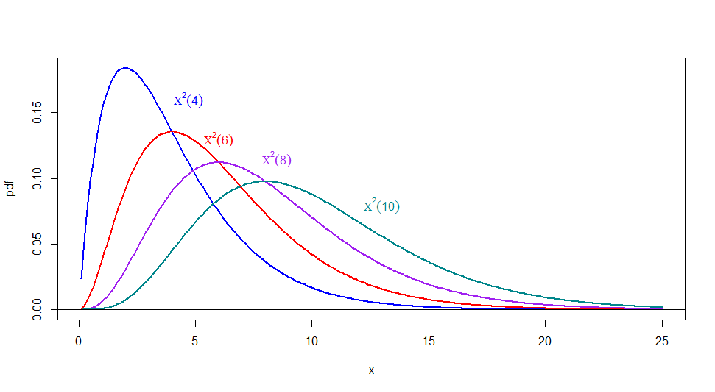
\includegraphics[height=2.6143in, width=4.6643in]{img/chisquared_pdfs__2.pdf}%
\end{figure}

Probabilities for Chi-squared distributions may be obtained from a table

\end{frame}%

\begin{frame}{\subsecname}

%\frametitle{Chi-squared table}


\begin{figure}[ptb]\centering
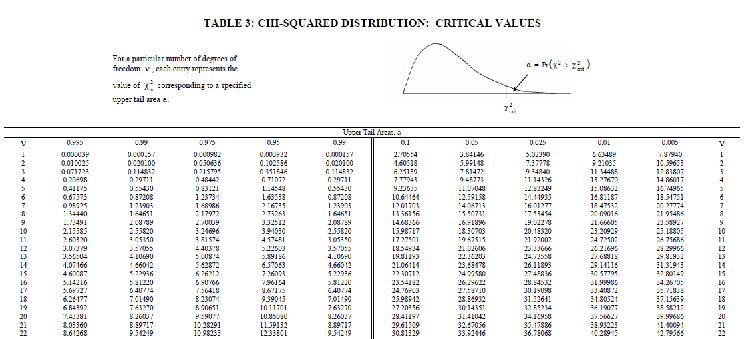
\includegraphics[height=2.2649in, width=4.9658in]{img/chisq_table__3.pdf}%
\end{figure}

\end{frame}%

\begin{frame}{\subsecname}

%\frametitle{Chi-squared table (illustration of its use)}

\begin{example}

Let $X$ be a chi-squared random variable with 10 degrees-of-freedom. What is the value of its \underline{upper fifth percentile}? \bigskip

By definition, the upper fifth percentile is the chi-squared value $x$ (lower case!!!) such that the probability to the right of $x$ is $0.05$ (so the upper tail area is $5\%$).  To find such an $x$ we use the chi-squared table: \medskip
\begin{itemize}
\item setting $\mathcal{V} = 10$ in the first column on the left and getting the corresponding row \medskip
\item finding the column headed by $P(X \geq x) = 0.05$. \medskip
\end{itemize}

Now, all we need to do is read the corresponding cell. What do we get? Well, the table tells us that the upper fifth percentile of a chi-squared random variable with 10 degrees of freedom is \textbf{18.30703}.
\end{example}
\end{frame}

%%%%%%%%%%%%%%%%%%%%%%%%%%%%%%%%%%%%%%%%%%%%%%%%%%%%%%%%%%%%%%%%%%%%%%%%%%%%%%%%
\subsection{The Student-t distribution}
%%%%%%%%%%%%%%%%%%%%%%%%%%%%%%%%%%%%%%%%%%%%%%%%%%%%%%%%%%%%%%%%%%%%%%%%%%%%%%%%

\begin{frame}{\subsecname}
  \begin{definition}
  If $Z\sim \N(0,1)$ and $Y\sim \chi ^{2}(v)$ are \textbf{independent}
  then%
  \begin{equation*}
  T=\frac{Z}{\sqrt{Y/v}}
  \end{equation*}%
  has a \textbf{Student-t} distribution with $v$ degrees of freedom. Write as $T\sim t_{v}$.
  \end{definition}
  \bigskip
  $T\sim t_{v}\,$\ can take any value in $\mathbb{R}$. Expected value and variance for $T\sim t_{v}$ are
  \begin{eqnarray*}
  E\left[ T\right] &=&0\text{, for }v>1 \\
  Var\left( T\right) &=&\frac{v}{v-2}\text{, for }v>2.
  \end{eqnarray*}
\end{frame}

\begin{frame}{\subsecname}
  \begin{remark}
  The pdf of $T\sim t_{v}$ is similar to a Normal (with mean zero) but with fatter tails. When $v$ is large (typically, $v \geq 120$) $t_{v}$ approaches $\N(0,1)$.
  \end{remark}

  \begin{figure}[ptb]\centering
  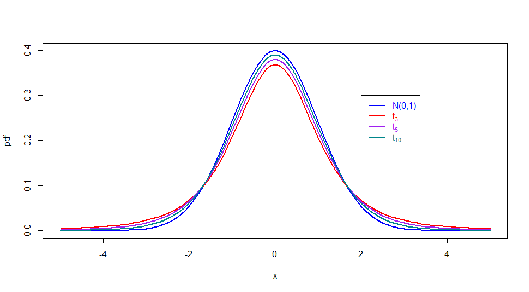
\includegraphics[height=1.9398in, width=3.5345in]{img/student_t__4.pdf}%
  \end{figure}
\end{frame}

\begin{frame}{\subsecname}
%\frametitle{Student-t table}

\begin{figure}[ptb]\centering
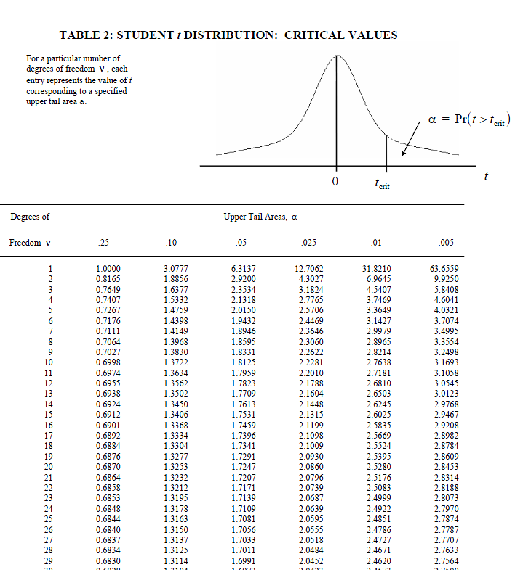
\includegraphics[height=3.8in, width=3.506in]{img/Student_t_table__5.pdf}%
\end{figure}

\end{frame}

%%%%%%%%%%%%%%%%%%%%%%%%%%%%%%%%%%%%%%%%%%%%%%%%%%%%%%%%%%%%%%%%%%%%%%%%%%%%%%%%
\subsection{The F distribution}
%%%%%%%%%%%%%%%%%%%%%%%%%%%%%%%%%%%%%%%%%%%%%%%%%%%%%%%%%%%%%%%%%%%%%%%%%%%%%%%%

\begin{frame}{\subsecname}
  \begin{definition}
  If $X\sim \chi ^{2}(v_{1})$ and $Y\sim \chi ^{2}(v_{2})$ are \textbf{%
  independent}, then%
  \begin{equation*}
  F=\frac{\frac{X}{v_{1}}}{\frac{Y}{v_{2}}},
  \end{equation*}%
  has an \textbf{F} distribution with $v_{1}$ `numerator' and $v_{2}$
  `denominator' degrees of freedom. Write as $F\sim F_{v_{1},v_{2}}$.
  \end{definition}

  $F\sim F_{v_{1},v_{2}}\,$\ can take only \textbf{positive }values. Expected value and variance for $F\sim F_{v_{1},v_{2}}$ (note that the order of the degrees of freedom is important!).
  \begin{eqnarray*}
  E\left[ F\right] &=&\frac{v_{2}}{v_{2}-2}\text{, for }v_{2}>2 \\
  Var\left( F\right) &=&\frac{2v_{2}^{2}\left( v_{1}+v_{2}-2\right) }{%
  v_{1}\left( v_{2}-2\right) ^{2}\left( v_{2}-4\right) }\text{, for }v_{2}>4.
  \end{eqnarray*}
\end{frame}

\begin{frame}{\subsecname}
  %\frametitle{Some F distributions}

  \begin{figure}[ptb]\centering
  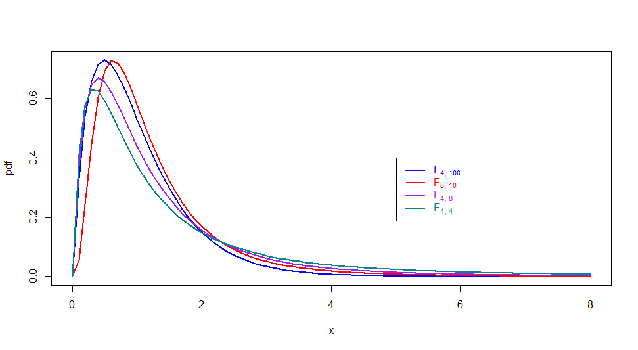
\includegraphics[height=2.3324in, width=4.2462in]{img/F-dist_pds__6.pdf}%
  \end{figure}%
\end{frame}%

\begin{frame}
  %\frametitle{F distribution table (5\% upper tail)}
  \begin{figure}[ptb]\centering
  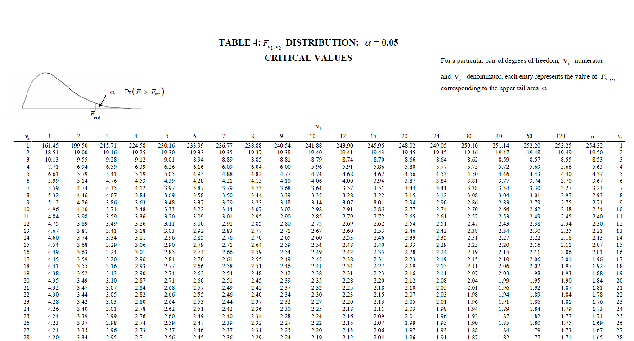
\includegraphics[height=2.2753in, width=4.2263in]{img/Fdist_table__7.pdf}%
  \end{figure}
\end{frame}%

%%%%%%%%%%%%%%%%%%%%%%%%%%%%%%%%%%%%%%%%%%%%%%%%%%%%%%%%%%%%%%%%%%%%%%%%%%%%%%%%
\subsection{The lognormal distribution}
%%%%%%%%%%%%%%%%%%%%%%%%%%%%%%%%%%%%%%%%%%%%%%%%%%%%%%%%%%%%%%%%%%%%%%%%%%%%%%%%

\begin{frame}{\subsecname}
  \begin{definition}
   $Y$ has a \textbf{lognormal distribution} when
   $$\ln \left( Y\right) =X$$
  has a Normal distribution. We write $Y\sim $ \emph{lognormal}$\left( \mu ,\sigma ^{2}\right) $.
  \end{definition}

  \medskip

  If $Y\sim $ \emph{lognormal}$\left( \mu ,\sigma ^{2}\right) $ then%
  \begin{eqnarray*}
  E\left[ Y\right] &=&\exp{ \left( \mu +\frac{1}{2}\sigma ^{2}\right)} \\
  Var(Y) &=&\exp{ \left( 2\mu +\sigma ^{2}\right)} \left( \exp{ \left( \sigma
  ^{2}\right)} -1\right).
  \end{eqnarray*}
\end{frame}

\begin{frame}{\subsecname}
  Let us just see some plots... more to come later...
  \begin{figure}[ptb]\centering
  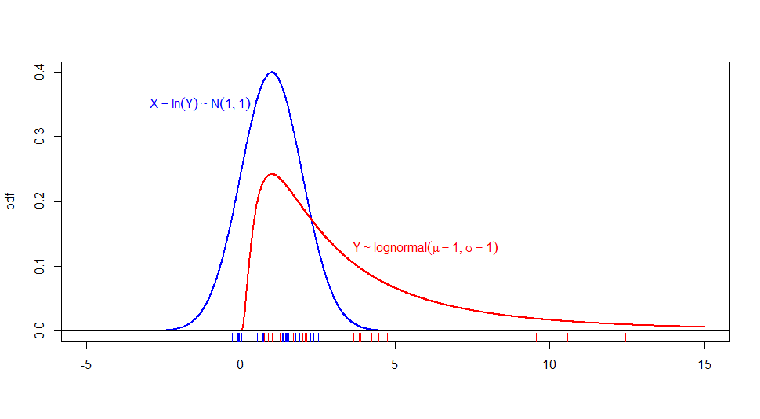
\includegraphics[height=2.4856in, width=4.5in]{img/lognormal_with_rug__8.pdf}%
  \end{figure}
\end{frame}

%%%%%%%%%%%%%%%%%%%%%%%%%%%%%%%%%%%%%%%%%%%%%%%%%%%%%%%%%%%%%%%%%%%%%%%%%%%%%%%%
\subsection{Exponential distribution}
%%%%%%%%%%%%%%%%%%%%%%%%%%%%%%%%%%%%%%%%%%%%%%%%%%%%%%%%%%%%%%%%%%%%%%%%%%%%%%%%

\begin{frame}{\subsecname}
  \begin{definition}
  Let $X$ be a  continuous random variable, having the following  characteristics:
  \begin{itemize}
  \item[--]       $X$ is defined on the positive real numbers $\left( 0;\infty \right) $ --- namely $\mathbb{R}^+$;
  \item[--]       the pdf and CDF are
  \bea
  f_X(x)=\lambda \exp{ -\lambda x},\lambda
  >0; &
  F_X(x)=1-\exp (-\lambda x); \nn \eea
  \end{itemize}
  then we say that $X$ has an exponential distribution. We write $X\sim$ \text{Exp$(\lambda)$}.
  \end{definition}

  For $X\sim$ \text{Exp$(\lambda)$} we have that:
  \begin{small}
  \bea
  E[X]=\int_{0}^{\infty }xf_X(x )dx= 1/\lambda & \text{and} &   Var(X)=\int_{0}^{\infty }x^{2}f_X(x )dx-E^{2}(X)=1/\lambda ^{2}. \nn
  \eea
  \end{small}

  \begin{remark}
  $X$ is typically applied to model the waiting time until an event occurs, when events are always occurring at a random rate $\lambda >0$. Moreover, the sum of independent exponential random variables has a Gamma distribution (see tutorial).
  \end{remark}
\end{frame}

\begin{frame}{\subsecname}
  %\frametitle{Exponential distribution}
  \begin{small}
  \begin{example}
  Let $X\sim$ \text{Exp}$(\lambda)$, with $\lambda =0.5$. Thus
  $$f_X(x) = \left\{ \begin{array}{ll}
  0.5 \exp (-0.5x) & x>0\\
  0 & \text{otherwise}
  \end{array} \right.$$
  Then, find the CDF.
  %
  \medskip

  For $x>0$, we have
  \begin{eqnarray*}
  F_{X}(x) & = & \int_{0}^{x}f_{X}(u)du\\
  & = & 0.5\Big( -2\exp (-0.5u)\Big) \bigl|_{u=0}^{u=x}\\
  & = & 0.5(-2\exp (-0.5x)+2\exp (0))\\
  & = & 1-\exp (-0.5x)
  \end{eqnarray*}

  so, finally,

  $$F_X(x) = \left\{ \begin{array}{ll}
  0 & x \leq 0 \\
  1-\exp (-0.5x)& x>0
  \end{array} \right.$$
  \end{example}
  \end{small}
\end{frame}

\begin{frame}{\subsecname}
  \begin{example} [continued]

  ...and a graphical illustration, with varying $\lambda$

  \begin{figure}[ptb]\centering
  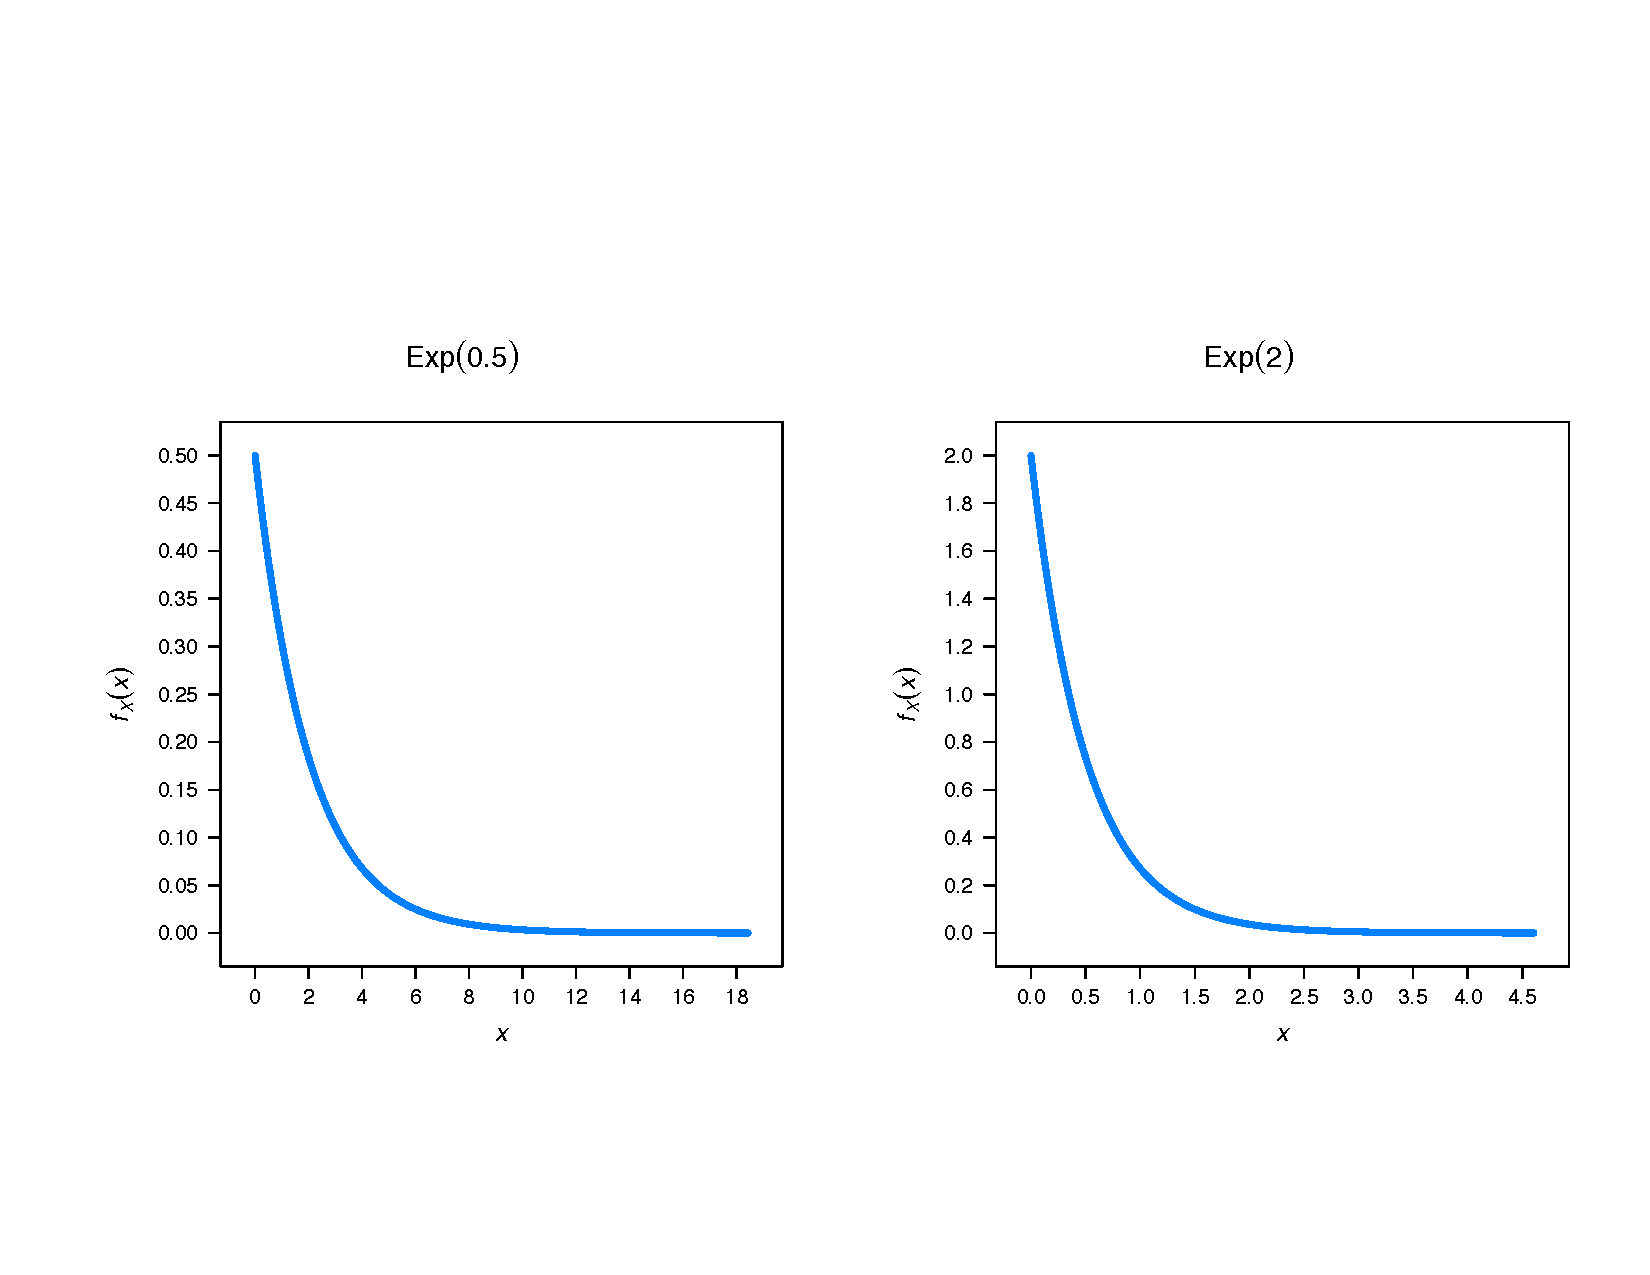
\includegraphics[height=2.4856in, width=4.5in]{img/Exp_Diego.pdf}%
  \end{figure}%

  \end{example}
\end{frame}

%%%%%%%%%%%%%%%%%%%%%%%%%%%%%%%%%%%%%%%%%%%%%%%%%%%%%%%%%%%%%%%%%%%%%%%%%%%%%%%%
\section{Variable Transformation}
%%%%%%%%%%%%%%%%%%%%%%%%%%%%%%%%%%%%%%%%%%%%%%%%%%%%%%%%%%%%%%%%%%%%%%%%%%%%%%%%


\begin{frame}{\secname}
  \begin{stepitemize}
  \item Consider a random variable $X$

  \item Suppose we are interested in $Y=\psi(X)$, where $\psi $ is a \textbf{%
  one to one function}

  \begin{stepitemize}
  \item A \textbf{function }$\psi \left( x\right) $\textbf{\ is one to one}
  (1-to-1) if there are no two numbers, $x_{1},x_{2}$ in the domain of $\psi $
  such that $\psi \left( x_{1}\right) =\psi \left( x_{2}\right) $ but $%
  x_{1}\neq x_{2}$.

  \item A sufficient condition for $\psi \left( x\right) $ to be 1-to-1 is
  that it be monotonically increasing (or decreasing) in $x$.

  \item Note that the \textbf{inverse} of a 1-to-1 function $y=\psi \left(
  x\right) $ is a 1-to-1 function $\psi^{-1}\left( y\right) $ such that
  \begin{equation*}
  \psi ^{-1}\left( \psi \left( x\right) \right) =x\text{ and }\psi \left( \psi
  ^{-1}\left( y\right) \right) =y.
  \end{equation*}
  \end{stepitemize}

  \item To transform $X$ to $Y$, we need to consider all the values $x$ that $%
  X $ can take

  \item We first transform $x$ into values $y=\psi (x)$
  \end{stepitemize}
\end{frame}

\begin{frame}{\secname}
  \framesubtitle{Transformation of discrete random variables}

  \begin{stepitemize}
  \item To transform a discrete random variable $X$, into the random variable $%
  Y=\psi (X)$, we transfer the probabilities for\textbf{\ each} $x$ to the values $%
  y=\psi \left( x\right) $:
  \begin{equation*}
  \begin{tabular}{l|cll|c}
  \multicolumn{2}{l}{\emph{Probability function for }$X$} &  &
  \multicolumn{2}{l}{\emph{Probability function for }$X$} \\
  &  &  &  &  \\
  $X$ & $\Pr \left(\{ X=x_{i} \}\right) =p_{i}$ &  & $Y$ & $\Pr \left(\{
  X=x_{i}  \}\right) =p_{i}$ \\ \cline{1-2}\cline{4-5}
  $x_{1}$ & $p_{1}$ & $\qquad \Rightarrow \qquad $ & $\psi (x_{1})$ & $p_{1}$
  \\
  $x_{2}$ & $p_{2}$ &  & $\psi (x_{2})$ & $p_{2}$ \\
  $x_{3}$ & $p_{3}$ &  & $\psi (x_{3})$ & $p_{3}$ \\
  $\vdots $ & $\vdots $ &  & $\vdots $ & $\vdots $ \\
  $x_{n}$ & $p_{n}$ &  & $\psi (x_{n})$ & $p_{n}$%
  \end{tabular}%
  \end{equation*}

  \item Note that this is equivalent to applying the function $\psi \left(
  \cdot \right) $ inside the probability statements:%
  \begin{eqnarray*}
  \Pr \left( \{ X=x_{i}  \}\right) &=&\Pr \left(  \{\psi \left( X\right) =\psi \left(
  x_{i}\right)  \} \right) \\
  &=&\Pr \left( \{ Y=y_{i} \} \right) \\
  &=&p_{i}
  \end{eqnarray*}
  \end{stepitemize}

\end{frame}


\begin{frame}{\secname}
\framesubtitle{Transformation of discrete random variables}
\begin{example} [option pricing]

Let us imagine that we are tossing a balanced coin ($p=1/2$), and when we get a ``Head'' ($H$) the stock price moves up of a factor $u$, but when we get a ``Tail'' ($T$) the price moves down of a factor $d$. We denote the price at time $t_1$  by $S_1(H)=u S_0 $ if the toss results in head ($H$), and by $S_1(T)=d S_0 $  if it results in tail ($T$). After the second toss, the price will be one of:
\begin{figure}[ptb]\centering
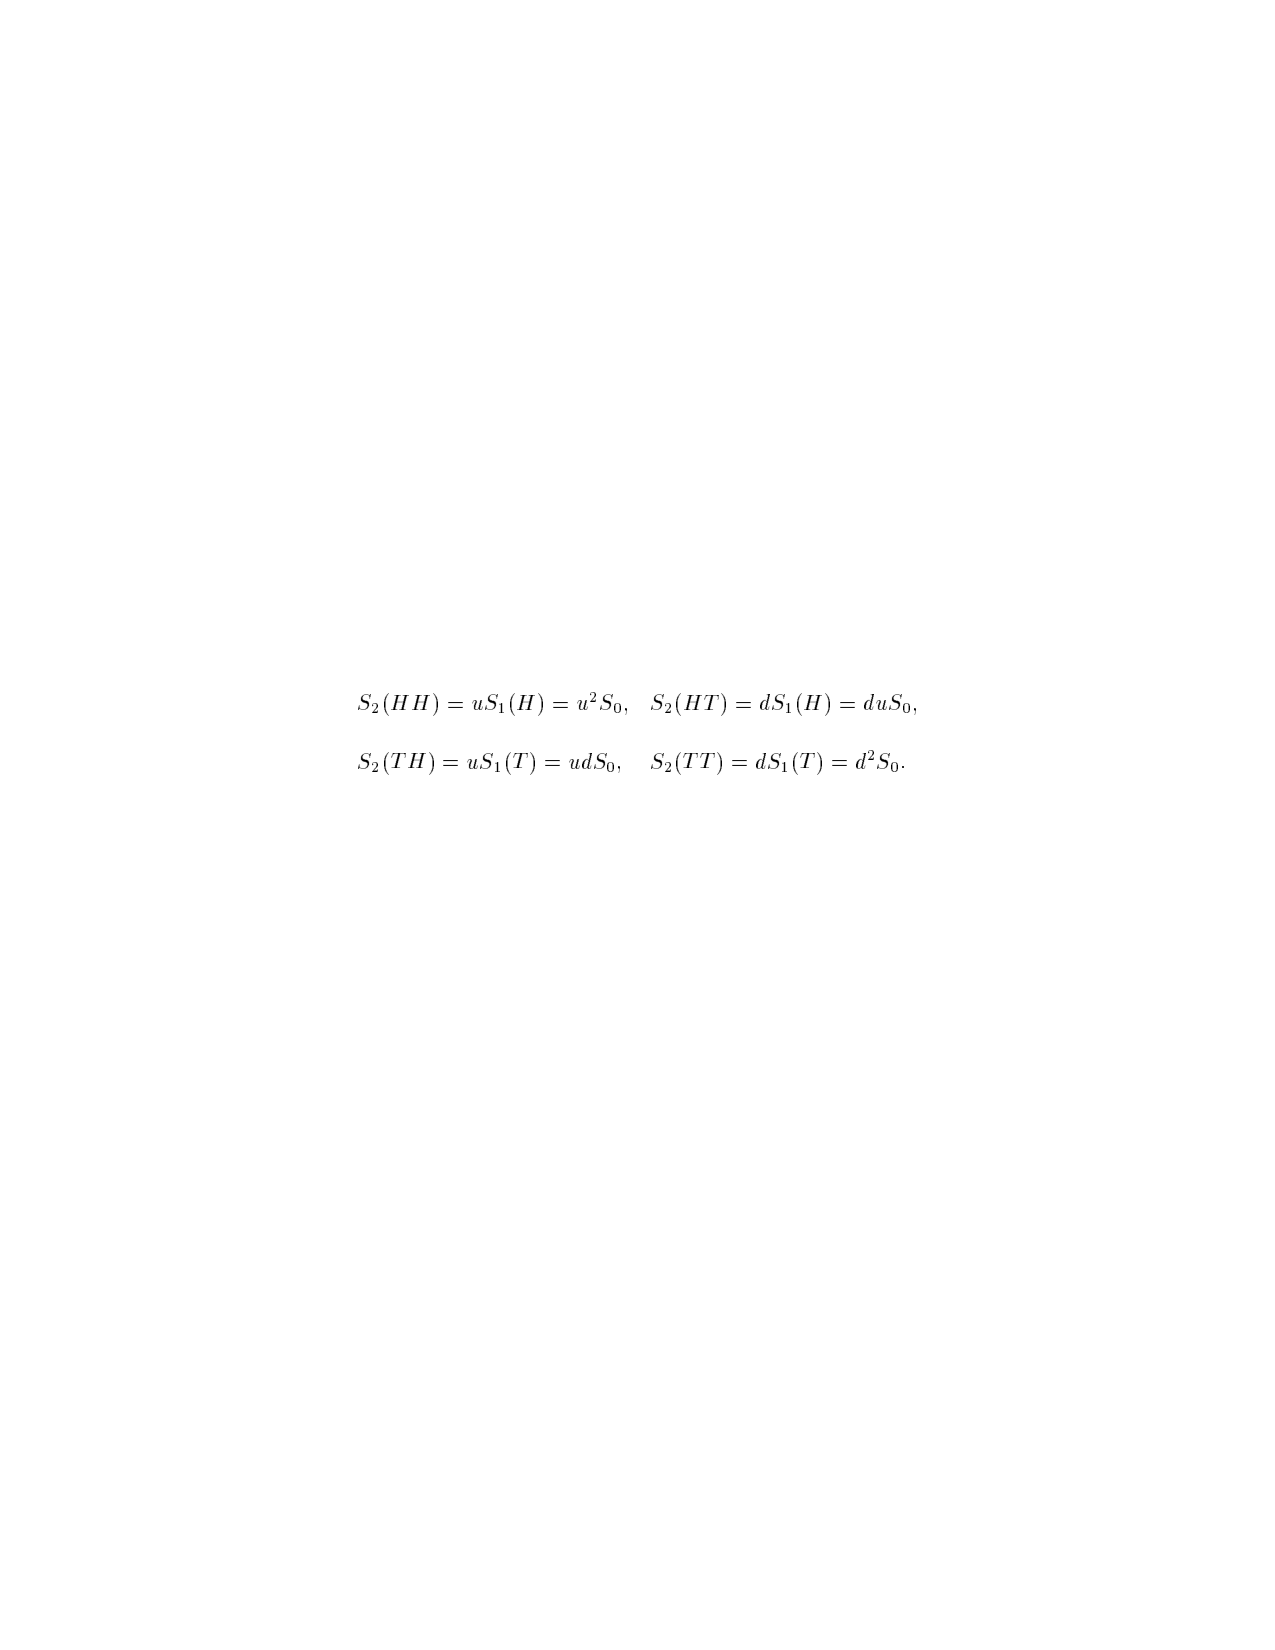
\includegraphics[height=0.75in, width=4in]{img/Shreve_Bin.pdf}%
\end{figure}%
Indeed, after two tosses, there are four possible coin sequences,
$$
\{HH,HT,TH,TT\}
$$
although not all of them result in different stock prices at time  $t_2$.
%
%% Define styles for bags and leafs
%\tikzstyle{bag} = [text width=2em, text centered]
%\tikzstyle{end} = []
%\begin{tikzpicture}[sloped]
%   \node (a) at ( 0,0) [bag] {$\$ A$};
%   \node (b) at ( 4,-1.5) [bag] {B};
%   \node (c) at ( 4,1.5) [bag] {C};
%   \node (d) at ( 8,-3) [bag] {D};
%   \node (e) at ( 8,0) [bag] {E};
%   \node (f) at ( 8,3) [bag] {F};
%   \draw [->] (a) to node [below] {$(1-p)$} (b);
%   \draw [->] (a) to node [above] {$P$} (c);
%   \draw [->] (c) to node [below] {$P^2$} (f);
%   \draw [->] (c) to node [above] {$(1-p)p$} (e);
%   \draw [->] (b) to node [below] {$(1-p)p$} (e);
%   \draw [->] (b) to node [above] {$(1-p)^2$} (d);
%\end{tikzpicture}
\end{example}
\end{frame}%





\begin{frame}{\secname}
\framesubtitle{Transformation of discrete random variables}
\begin{example}[continued]
Let us set $S_0=1$, $u=2$ and $d=1/2$: we represent the price evolution by a tree:


%
%% Define styles for bags and leafs
\tikzstyle{bag} = [text width=8em, text centered]
\tikzstyle{end} = []
\begin{tikzpicture}[sloped]
   \node (a) at ( 0,0) [bag] {$\$ 1$};
   \node (b) at ( 4,-1.5) [bag] {$\$ d =\$ 0.5$};
   \node (c) at ( 4,1.5) [bag] {$\$ u= \$ 2$};
   \node (d) at ( 8,-3) [bag] {$\$ d^2= \$ 0.25$};
   \node (e) at ( 8,0) [bag] {$\$ ud= \$ du = \$ 1$};
   \node (f) at ( 8,3) [bag] {$\$ u^2=\$ 4$};
   \draw [->] (a) to node [below] {$(1-p)$} (b);
   \draw [->] (a) to node [above] {$p$} (c);
   \draw [->] (c) to node [below] {$p^2$} (f);
   \draw [->] (c) to node [above] {$(1-p)p$} (e);
   \draw [->] (b) to node [below] {$(1-p)p$} (e);
   \draw [->] (b) to node [above] {$(1-p)^2$} (d);
\end{tikzpicture}
\end{example}
\end{frame}%



\begin{frame}{\secname}
\framesubtitle{Transformation of discrete random variables}
  \begin{example}[continued]
  Now consider an European option call with maturity $t_2$ and strike price $K=0.5$, whose random pay-off at $t_2$ is $C=\max(0;S_2-0.5)$. Thus,
  \begin{eqnarray*}
  C(HH)=\max(0;4-0.5)=\$ 3.5 & C(HT)=\max(0;1-0.5)=\$ 0.5 \\
  C(TH)=\max(0;1-0.5)=\$ 0.5 & C(TT)=\max(0;0.25-0.5)=\$ 0.
  \end{eqnarray*}
  Thus at maturity $t_2$ we have
  \begin{equation*}
  \begin{tabular}{l|cll|c}
  \multicolumn{2}{l}{\emph{Probability function for }$S_2$} &  &
  \multicolumn{2}{l}{\emph{Probability function for }$C$} \\
  &  &  &  &  \\
  $S_2$ & $\Pr \left(\{ X=x_{i} \}\right) =p_{i}$ &  & $C$ & $\Pr \left(\{
  C=c_{i}  \}\right) =p_{i}$ \\ \cline{1-2}\cline{4-5}
  $\$ u^2$ & $p^2$ & $\qquad \Rightarrow \qquad $ & $\$ 3.5$ & $p^2$
  \\
  $\$ ud$ & $2p(1-p)$ &  & $\$ 0.5$ & $2p(1-p)$ \\
  %$\$ du$ & $(1-p)p$ &  & $\$ 0.5$ & $(1-p)p$ \\
  $\$ d^2$ & $(1-p)^2$  &  & $\$ 0$ & $(1-p)^2$%
  \end{tabular}%
  \end{equation*}
  \tiny{Since $ud=du$ the corresponding values of $S_2$ and $C$ can be aggregated, without loss of info.}
  \end{example}
\end{frame}%


\begin{frame}{\secname}
\framesubtitle{Transformation of variables using the CDF}

  \begin{stepitemize}
  \item We can use the same logic for CDF probabilities, whether the random
  variables are\textbf{\ discrete or continuous}

  \item Let $Y=\psi \left( X\right) $ with $\psi \left( x\right) $ 1-to-1 and
  monotone increasing. Then
  \begin{eqnarray*}
  F_{Y}\left( y\right) &=&\Pr \left( \{ Y\leq y \}\right) \\
  &=&\Pr \left( \{ \psi \left( X\right) \leq y \} \right) =\Pr \left( \{ X\leq \psi
  ^{-1}\left( y\right) \} \right) \\
  &=&F_{X}\left( \psi ^{-1}\left( y\right) \right)
  \end{eqnarray*}

  \begin{example}
  Let $Y=\psi \left( X\right) =\exp{ X} $ where $%
  X\sim F_X$ on all values $x\in
  %TCIMACRO{\U{211d} }%
  %BeginExpansion
  \mathbb{R}
  %EndExpansion
  $%
  \begin{eqnarray*}
  F_{Y}\left( y\right) &=&\Pr \left( \{ Y\leq y \} \right) \\
  &=&\Pr \left( \{ \exp{  X} \leq y \} \right) =\Pr \left( \{ X\leq \ln
  \left( y\right) \} \right) \\
  &=&F_{X}\left( \ln \left( y\right) \right) \text{ only for }y>0\text{.}
  \end{eqnarray*}
  \end{example}

  %\item True whether $X$ (and hence $Y$) are continuous or discrete random
  %variables.
  \end{stepitemize}

  %TCIMACRO{\TeXButton{EndFrame}{\end{frame}}}%
  %BeginExpansion
\end{frame}%

\begin{frame}{\secname}
  \framesubtitle{Function 1-to-1 and monotone decreasing}

  \begin{stepitemize}
  \item Monotone decreasing functions work in a similar way, but require
  changing of the inequality sign

  \item Let $Y=\psi \left( X\right) $ with $\psi \left( x\right) $ 1-to-1 and
  \textbf{monotone decreasing}. Then
  \begin{eqnarray*}
  F_{Y}\left( y\right) &=&\Pr \left( \{ Y\leq y \} \right) \\
  &=&\Pr \left( \{ \psi \left( X\right) \leq y \} \right) =\Pr \left( \{ X\geq \psi
  ^{-1}\left( y\right) \} \right) \\
  &=&1-F_{X}\left( \psi ^{-1}\left( y\right) \right)
  \end{eqnarray*}

  \end{stepitemize}
  \begin{example}
  Example: let $Y=\psi \left( X\right) =-\exp X $ where $%
  X\sim F_X$ on all values $x\in
  %TCIMACRO{\U{211d} }%
  %BeginExpansion
  \mathbb{R}
  %EndExpansion
  $%
  \begin{eqnarray*}
  F_{Y}\left( y\right) &=&\Pr \left( \{ Y\leq y \}\right) =\Pr \left( \{ -\exp ^
  X \leq y \} \right) \\
  &=&\Pr \left( \{ \exp X \geq -y \} \right) =\Pr \left( \{ X\geq \ln
  \left( -y\right) \} \right) \\
  &=&1-F_{X}\left( \ln \left( -y\right) \right) \text{ only for }y<0\text{.}
  \end{eqnarray*}
  \end{example}
\end{frame}


\begin{frame}{\secname}
  \framesubtitle{Transformation of continuous RV through pdf}

  \begin{stepitemize}
  \item For continuous random variables, if $\psi \left( x\right) $ 1-to-1 and
  monotone \textbf{increasing}, we have%
  \begin{equation*}
  F_{Y}\left( y\right) =F_{X}\left( \psi ^{-1}\left( y\right) \right)
  \end{equation*}

  \item Notice this implies that the pdf of $Y=\psi \left( X\right) $ must
  satisfy%
  \begin{eqnarray*}
  f_{Y}\left( y\right) &=&\frac{dF_{Y}\left( y\right) }{dy}=\frac{dF_{X}\left(
  \psi ^{-1}\left( y\right) \right) }{dy} \\
  &=&\frac{dF_{X}\left( x\right) }{dx}\times \frac{d\psi ^{-1}\left( y\right)
  }{dy}\qquad \text{{\small (chain rule)}} \\
  &=&f_{X}\left( x\right) \times \frac{d\psi ^{-1}\left( y\right) }{dy}\qquad
  \text{{\small (derivative of CDF (of }}X\text{){\small \ is pdf)}} \\
  &=&f_{X}\left( \psi ^{-1}\left( y\right) \right) \times \frac{d\psi
  ^{-1}\left( y\right) }{dy}\qquad \text{{\small (substitute }}x=\psi
  ^{-1}\left( y\right) \text{{\small )}}
  \end{eqnarray*}
  \end{stepitemize}

\end{frame}

\begin{frame}{\secname}
  \framesubtitle{Transformation of continuous RV through pdf}

  \begin{stepitemize}
  \item What happens when $\psi \left( x\right) $ 1-to-1 and monotone \textbf{%
  decreasing}? We have%
  \begin{equation*}
  F_{Y}\left( y\right) =1-F_{X}\left( \psi ^{-1}\left( y\right) \right)
  \end{equation*}

  \item So now the pdf of $Y=\phi \left( X\right) $ must satisfy
  \begin{eqnarray*}
  f_{Y}\left( y\right) &=&\frac{dF_{Y}\left( y\right) }{dy}=-\frac{%
  dF_{X}\left( \psi ^{-1}\left( y\right) \right) }{dy} \\
  &=&-f_{X}\left( \psi ^{-1}\left( y\right) \right) \times \frac{d\psi
  ^{-1}\left( y\right) }{dy}\qquad \text{{\small (same reasons as before)}}
  \end{eqnarray*}

  \item but $\frac{d\psi ^{-1}\left( y\right) }{dy}<0$ since here $\psi \left(
  \cdot \right) $ is monotone decreasing, hence we can write%
  \begin{equation*}
  f_{Y}\left( y\right) =f_{X}\left( \psi ^{-1}\left( y\right) \right) \times
  \left\vert \frac{d\psi ^{-1}\left( y\right) }{dy}\right\vert
  \end{equation*}

  \item This expression (called Jacobian-formula) is valid for $\psi \left( x\right) $ 1-to-1 and
  monotone (whether increasing or decreasing)
  \end{stepitemize}
\end{frame}

\begin{frame}{\secname}
  \framesubtitle{Transformation of continuous RV through pdf }

  \begin{example}
  \begin{stepitemize}
  \item So what is the pdf for the lognormal distribution?

  \item Recall that $Y$ has a \textbf{lognormal distribution} when $\ln \left(
  Y\right) =X$ has a Normal distribution

  \item $\Rightarrow $ if $X\sim \N\left( \mu ,\sigma ^{2}\right) ,$ then $%
  Y=\exp X \sim $ \emph{lognormal}$\left( \mu ,\sigma ^{2}\right) $

  \begin{stepitemize}
  \item Corresponding to $\psi \left( x\right) =\exp x$ and $\psi
  ^{-1}\left( y\right) =\ln (y)$
  \end{stepitemize}

  \item The \emph{pdf} of $X$ is
  \begin{equation*}
  f_{X}\left( x\right) =\frac{1}{\sqrt{2\pi \sigma ^{2}}}\exp{ \left\{ -\frac{1%
  }{2\sigma ^{2}}\left( x-\mu \right) ^{2}\right\}}
  \end{equation*}%
  for any $-\infty <x<\infty $

  \item Using $\psi \left( x\right) =\exp x$ we know we'll have possible
  values for $Y$ only on $0<y<\infty $
  \end{stepitemize}
  \end{example}
\end{frame}

\begin{frame}{\secname}
  \framesubtitle{Transformation of continuous RV through pdf }
  \begin{example}[continued]
  \begin{stepitemize}
  \item We know that
  \begin{equation*}
  f_{Y}\left( y\right) =f_{X}\left( \psi ^{-1}\left( y\right) \right) \times
  \left\vert \frac{d\psi ^{-1}\left( y\right) }{dy}\right\vert
  \end{equation*}

  \item And since $\psi ^{-1}\left( y\right) =\ln (y)$ then
  \begin{equation*}
  \left\vert \frac{d\psi ^{-1}\left( y\right) }{dy}\right\vert =\left\vert
  \frac{1}{y}\right\vert
  \end{equation*}

  \item $\Rightarrow $ the \emph{pdf} of $Y$ is
  \begin{equation*}
  f_{Y}\left( y\right) =\frac{1}{y\sqrt{2\pi \sigma ^{2}}}\exp{ \left\{ -\frac{1%
  }{2\sigma ^{2}}\left( \ln (y)-\mu \right) ^{2}\right\}}
  \end{equation*}
  for any $0<y<\infty $
  \end{stepitemize}
  \end{example}
\end{frame}

\begin{frame}{\secname}
  \begin{example}[continued]
  \begin{stepitemize}
  \item Both the Normal and the lognormal are characterized by
  only two parameters ($\mu$ and $\sigma$). The \emph{median} of the lognormal distribution is $\exp{
  \mu } $, since $$
  \Pr \left( \{ X\leq \mu \} \right) = 0.5,
  $$
  and hence%
  \begin{eqnarray*}
  0.5 &=&\Pr \left(\{ X\leq \mu \}\right) \\
  &=&\Pr \left( \{\exp{X} \leq \exp{ \mu }\} \right) \\
  &=&\Pr \left( \{Y\leq \exp{ \mu }\} \right).
  \end{eqnarray*}
  \end{stepitemize}
  \end{example}
  More generally, for $\alpha\in[0,1]$, the $\alpha$-th quantile of a r.v. $X$ is the value $x_\alpha$ such that $P(\{X \leq x_\alpha\})\geq\alpha$. If $X$ si a continuous r.v.  we can set $P(\{X \leq x_\alpha\})=\alpha$ (as we did, e.g., for the lognormal).
\end{frame}

\begin{frame}{\secname}
\framesubtitle{A caveat }

  When $X$ and $Y$ are two random variables, we should pay attention to their transformations. For instance, let us consider
  $$
  X\sim \mathcal{N}(\mu,\sigma^2) \quad \text{and}  \quad Y\sim Exp(\lambda).
  $$
  Then, let's transform $X$ and $Y$

  \begin{itemize}
  \item  in a linear way: $Z=X+Y$. We know that
  $$
  E[Z] = E[X+Y] = E[X] + E[Y]
  $$
  %so we can rely on the linearity of the expected value.
  \item in a nonlinear way $W = X/Y$. One can show that
  $$\color{red}
  E[W] = E\left[\frac{X}{Y}\right] \neq \frac{E[X]}{E[Y]}. \color{black}
  $$
  %so, we cannot rely on the linearity of the expected value.
   \end{itemize}
\end{frame}

\begin{frame}{{\secname}}
  \framesubtitle{The big picture}

  Despite exotic names, the common distributions relate to each other in intuitive and interesting ways. Several follow naturally from the Bernoulli distribution, for example.

  \begin{figure}[ptb]\centering
  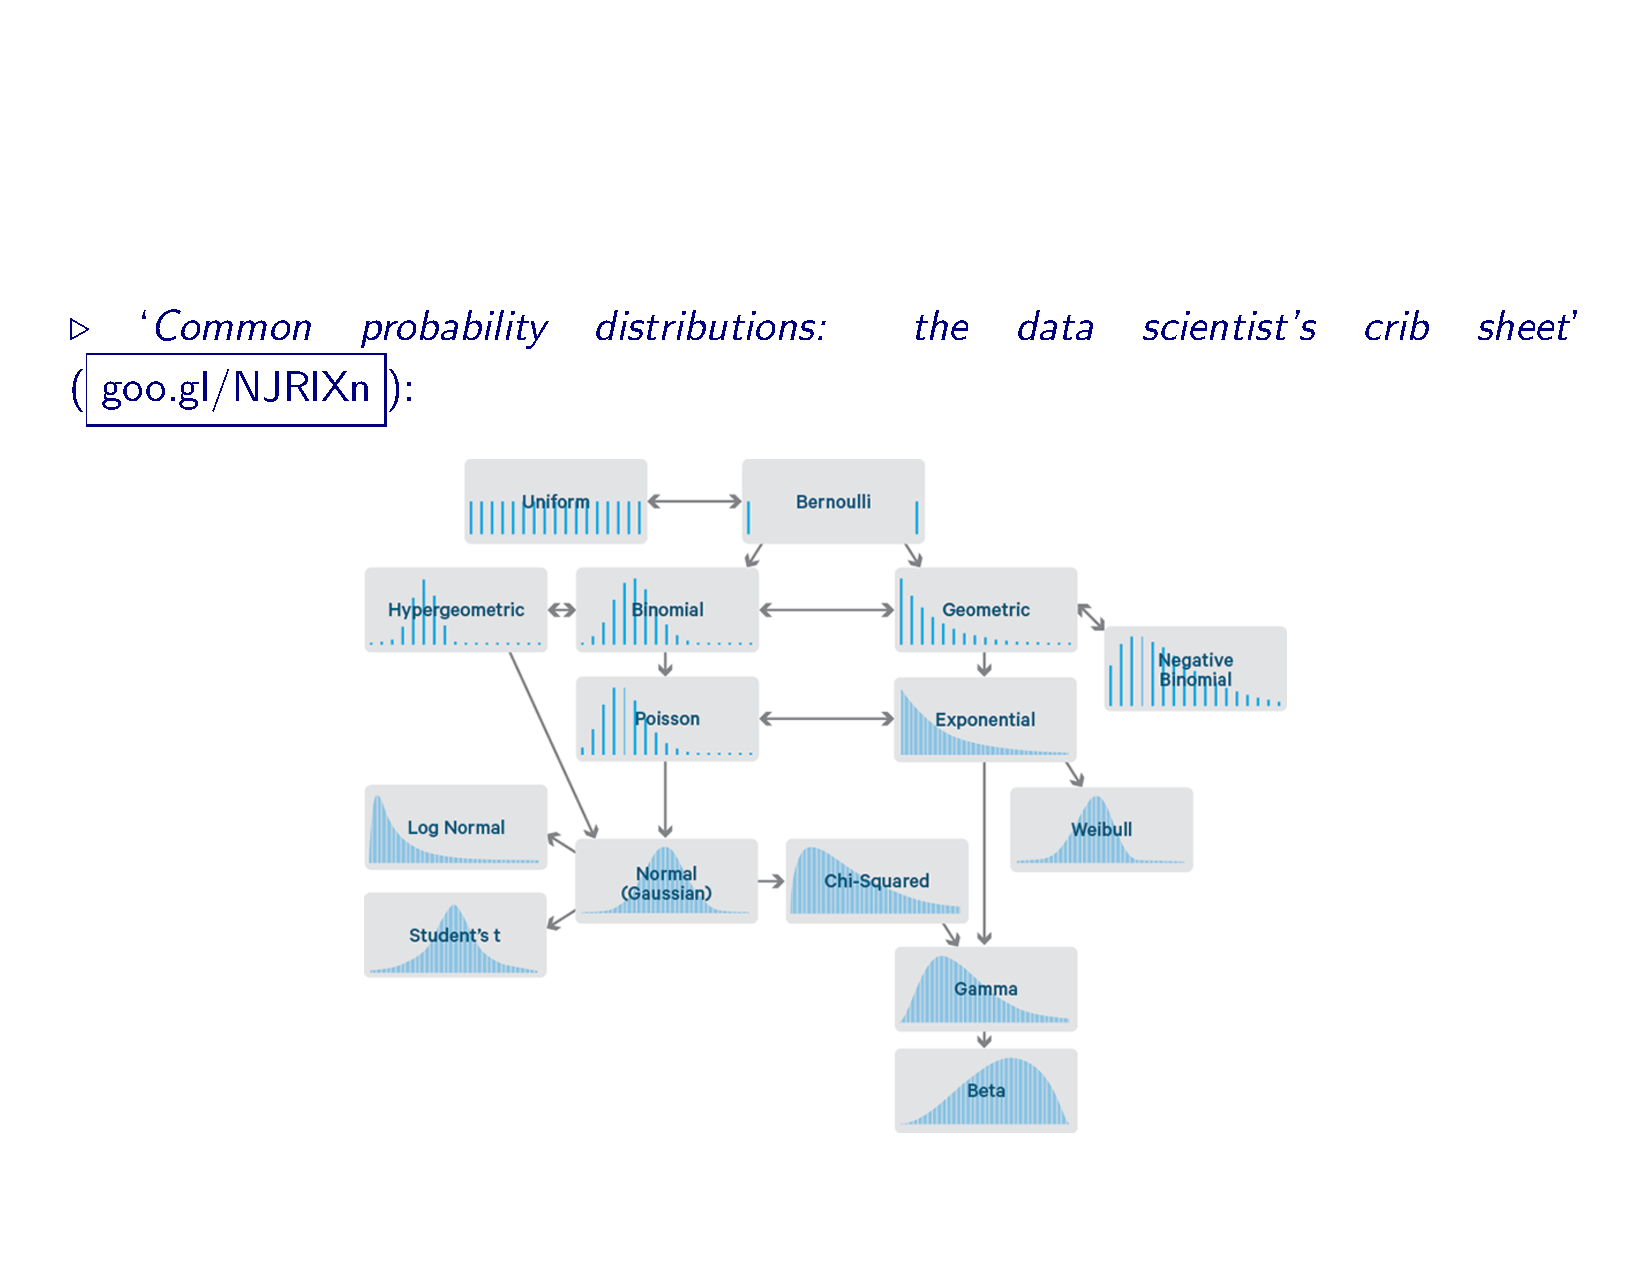
\includegraphics[height=2.3in, width=4.5in]{img/RelRVs_Diego.pdf}%
  \end{figure}
\end{frame}

\end{document}
